% -*- coding: utf-8 -*-

\begin{chapter}{Численные модели}\label{chap:15}
% \chapter{Numerical Models}
Как уже было сказано ранее, найти аналитическое решение уравнений
движения для типичных океанских потоков невозможно. Возникающие проблемы
связаны с нелинейными членами уравнений, 
турбулентностью\index{турбулентность!в численных моделях}, а также с
необходимостью учитывать реальную топографию дна и форму береговой
линии. Мы уже видели, насколько проблематично описать динамику океана,
используя только натурные наблюдения. Конечно, спутниковые данные дают
нам представление о состоянии практически всего океана с временным
шагом в несколько дней. Но речь в этом случае идет только об
определенных процессах, происходящих либо на поверхности океана, либо на
сравнительно небольшой глубине.
Судовые измерения и данные дрейфующих буев позволяют наблюдать большее 
количество интересующих параметров и на б\'{о}льших глубинах, но плотность
покрытия океана при этом оставляет желать лучшего.
Таким образом, остается единственный практически пригодный
выход~--- численное моделирование глобальной системы
океанических течений. Ниже мы рассмотрим
точность\index{точность!численных моделей} и адекватность различных моделей.
При этом следует не забывать, что хоть это всего лишь модели, они 
предоставляют весьма детальную и реалистичную картину океана.
%
% We saw earlier that analytic solutions of the equations of motion are
% impossible to obtain for typical oceanic flows. The problem is due to
% non-linear terms in the equations of motion,
% turbulence\index{turbulence!in numerical models}, and the need for
% realistic shapes for the sea floor and coastlines. We have also seen
% how difficult it is to describe the ocean from
% measurements. Satellites can observe some processes almost everywhere
% every few days. But they observe only some processes, and only near or
% at the surface. Ships and floats can measure more variables, and
% deeper into the water, but the measurements are sparse. Hence,
% numerical models provide the only useful, global view of ocean
% currents. Let's look at the accuracy\index{accuracy!numerical models}
% and validity of the models, keeping in mind that although they are
% only models, they provide a remarkably detailed and realistic view of
% the ocean.

\begin{section}{Пределы применимости моделей}
% \section{Introduction--Some Words of Caution}
\index{численные модели!ограничения}%
Математические модели океанических течений, безусловно, обладают массой
преимуществ. Они имитируют течения в реальном океане с реальным
рельефом дна, учитывают вязкость жидкости и нелинейные компоненты уравнений
движения. Также модели можно использовать для прогнозирования динамики
океана в будущем. Возможно, самым важным их свойством будет то, что модели 
позволяют провести интерполяцию данных, полученных с судов, дрейфующих
буев\index{дрейфующий буй!и численные модели} и спутников.
%
% \index{numerical models!limitations of}Numerical models of ocean
% currents have many advantages. They simulate flows in realistic ocean
% basins with a realistic sea floor. They include the influence of
% viscosity and non-linear dynamics. And they can calculate possible
% future flows in the ocean. Perhaps, most important, they interpolate
% between sparse observations of the ocean produced by ships,
% drifters\index{drifters!and numerical models}, and satellites.

Однако, при моделировании также можно столкнуться с рядом затруднений. 
<<С одной стороны находятся фундаментальные законы физики, с другой~---
методы вычислений, призванные вдохнуть в них жизнь, а между ними~---
пропасть>> (Berlinski, 1996). Модель никогда не будет
в состоянии дать полную картину реальных океанических течений даже при
условии, что интегрирование уравнений проделано без погрешности. Возникающие
при этом проблемы имеют различную природу.
%
% Numerical models are not without problems. ``There is a world of
% difference between the character of the fundamental laws, on the one
% hand, and the nature of the computations required to breathe life into
% them, on the other''---Berlinski (1996). The models can never give
% complete descriptions of the oceanic flows even if the equations are
% integrated accurately. The problems arise from several sources.

\emph{Дискретные уравнения не идентичны непрерывным.}  
В гл.~\ref{chap:7} были получены дифференциальные уравнения движения 
сплошной текучей среды. В математических моделях используется алгебраическая
аппроксимация этих уравнений. Мы предполагаем, что океан представим в виде
некоторого конечного множества точек, образующих сетку, время~--- дискретно,
а значения скоростей течений, давления, температуры и солёности в заданной 
точке могут быть вычислены по значениям данных параметров в некоторой 
окрестности в предыдущие моменты времени. Известный математик 
Иан Стюарт указывает, что (Ian Stewart,1992):
%
% \textit{Discrete equations are not the same as continuous equations.}
% In Chapter 7 we wrote down the differential equations describing the
% motion of a continuous fluid. Numerical models use algebraic
% approximations to the differential equations. We assume that the ocean
% basins are filled with a grid of points, and time moves forward in
% tiny steps. The value of the current, pressure, temperature, and
% salinity are calculated from their values at nearby points and
% previous times. Ian Stewart (1992), a noted mathematician, points out
% that
\begin{quote}
Дискретизация необходима при машинных вычислениях, так что избежать ее 
невозможно. Суть затруднений в том, что динамика дискретной системы
достаточно слабо связана с непрерывной (в самом деле, динамика дискретных
систем куда более богата), так что использование аппроксимации может приводить 
к появлению ложных решений.
%
% Discretization is essential for computer implementation and cannot be
% dispensed with. The essence of the difficulty is that the dynamics of
% discrete systems is only loosely related to that of continuous
% systems---indeed the dynamics of discrete systems is far richer than
% that of their continuous counterparts---and the approximations
% involved can create spurious solutions.
\end{quote}

\emph{Трудности при расчете турбулентности\index{турбулентность!расчеты}.}  
Численные модели предоставляют информацию о значении какого-либо
параметра только в узлах сетки, но не в промежутках между ними. 
Поскольку океан турбулентен, любая его модель, способная воспроизводить
турбулентные явления, должна обладать пространственным разрешением сетки 
порядка миллиметров, а временным~--- порядка миллисекунд.
%
% \textit{Calculations of turbulence\index{turbulence!calculation of}
% are difficult.} Numerical models provide information only at grid
% points of the model. They provide no information about the flow
% between the points. Yet, the ocean is turbulent, and any oceanic model
% capable of resolving the turbulence needs grid points spaced
% millimeters apart, with time steps of milliseconds.

Практически применимые модели океана имеют анизотропную пространственную сетку 
с шагом порядка сотен километров по горизонтали и от десятков до сотен
метров по вертикали. Таким образом, турбулентность\index{турбулентность!расчет} 
как таковая не рассчитывается напрямую, но ее влияние учитывается 
через параметры модели. Холлоуэй дал краткое описание этой
проблемы (Holloway, 1994):
%
% Practical ocean models have grid points spaced tens to hundreds of
% kilometers apart in the horizontal, and tens to hundreds of meters
% apart in the vertical.  This means that
% turbulence\index{turbulence!calculation of} cannot be calculated
% directly, and the influence of turbulence must be
% parameterized. Holloway (1994) states the problem succinctly:
\begin{quotation}
Модели океанических процессов обладают меньшим (примерно на 20 порядков)
количеством степеней свободы, чем реальный океан. Мы пытаемся скомпенсировать
этот факт, используя <<eddy-viscous goo>>, при помощи которой мы пытаемся
покрыть все перемещения, не превышающие избранного нижнего предела масштабов
моделируемых явлений. (We also use non-conservative numerics.) 
Это напоминает попытку поставить перегородку в ящик с воздухом так,
чтобы молекулы воздуха не проникали в отгороженное
пространство. Наши модели океана не в состоянии овладеть большинством
степеней свободы, присущих реальному океану, попросту потому, что модели
их не включают.
%
% Ocean models retain fewer degrees of freedom than the actual ocean (by
% about 20 orders of magnitude). We compensate by applying `eddy-viscous
% goo' to squash motion at all but the smallest retained scales. (We
% also use non-conservative numerics.) This is analogous to placing a
% partition in a box to prevent gas molecules from invading another
% region of the box. Our oceanic models cannot invade most of the real
% oceanic degrees of freedom simply because the models do not include
% them.

Но если мы по объективным причинам не в состоянии сделать <<правильно>>, 
не лучше ли в таком случае вообще ничего не делать? Это не выход. 
<<Не делать ничего>> означает продолжать использовать понятие viscous goo и 
мечтать о более мощных компьютерах. Можем ли мы найти лучший выход?
Например, не сможем ли мы угадать состояние с большей энтропией, в которое
вихри будут стремиться привести океан (данная тенденция будет противостоять
приложенным извне силам и диссипации)?
%
% Given that we cannot do things `right', is it better to do nothing?
% That is not an option. `Nothing' means applying viscous goo and
% wishing for the ever bigger computer. Can we do better? For example,
% can we guess a higher entropy configuration toward which the eddies
% tend to drive the ocean (that tendency to compete with the imposed
% forcing and dissipation)?
\end{quotation}

Под термином <<степени свободы>> Холлоуэй понимает любые возможные
движения в океане: от мельчайших волн и турбулентности\index{турбулентность} 
до крупнейших океанических течений. Проведем некоторые подсчеты. Нам
известно, что турбулентность океана проявляется в виде вихрей размером от
нескольких миллиметров и более. Чтобы полностью описать такой океан, нам потребуется
модель с шагом пространственной сетки~$1\mm$ и временным шагом около~$1\msec$.
Таким образом, модель должна иметь сетку размером 
$\degrees{360} \times \degrees{180} \times (111\text{~км/градус})^2 
 \times 10^{12}\text{~(мм/км)}^2  \times 3\text{~км} \times 10^6\text{~(мм/км)} 
 = 2.4 \times 10^{27}$~точек, чтобы представить океан толщиной~$3\km$, 
покрывающий всю поверхность Земли. Глобальная модель Parallel Ocean Program, 
описанная ниже, имеет всего лишь $2.2 \times 10^7$~точек. Таким
образом, для описания реального океана потребуется в $10^{20}$~раз больше
точек~--- это и есть те самые отсутствующие $10^{20}$~степеней свободы.
%
% By ``degrees of freedom'' Holloway means all possible motions from the
% smallest waves and turbulence\index{turbulence} to the largest
% currents. Let's do a calculation.  We know that the ocean is turbulent
% with eddies as small as a few millimeters. To completely describe the
% ocean we need a model with grid points spaced 1 mm apart and time
% steps of about 1 ms. The model must therefore have 360\degrees
% $\times$ 180\degrees $\times$ (111 km/degree)$^2 \times 10^{12}$
% (mm/km)$^2 \times$ 3 km $\times 10^6$ (mm/km) $= 2.4 \times 10^{27}$
% data points for a 3 km deep ocean covering the globe. The global
% Parallel Ocean Program Model described in the next section has $2.2
% \times 10^7$ points. So we need $10^{20}$ times more points to
% describe the real ocean. These are the missing $10^{20}$ degrees of
% freedom.

\emph{Практически применимые модели должны быть проще, чем реальный океан.}
Модели океана должны соответствовать возможностям доступных компьютеров. 
Это значит, что океанологи будут и дальше вносить в них различные упрощения.
Мы пользуемся приближениями Буссинеска\index{Буссинеска приближение} и
гидростатики, а также широко применяем 
уравнения, интегрированные в вертикальном направлении~--- уравнения 
мелкой воды (Haidvogel and Beckmann, 1999: 37). Необходимость
подобных шагов диктуется невозможностью просчитать наиболее детализированные 
модели циркуляции океана на протяжении нескольких тысяч лет, что требуется 
для определения роли океана в формировании климата.
%
% \textit{Practical models must be simpler than the real ocean.} Models
% of the ocean must run on available computers. This means
% oceanographers further simplify their models. We use the hydrostatic
% and Boussinesq approximations\index{Boussinesq approximation}, and we
% often use equations integrated in the vertical, the shallow-water
% equations (Haidvogel and Beckmann, 1999: 37). We do this because we
% cannot yet run the most detailed models of oceanic circulation for
% thousands of years to understand the role of the ocean in climate.

%% В оригинале отсутствует:
%% \emph{Неизвестные начальные условия.} 
%% Как нам инициировать (откалибровать) модель? Мы не можем достаточно
%% точно определить скорость и плотность в какой-либо точке океана,
%% которая могла бы послужить отправной точкой, началом отсчета
%% модели. Самое большее, что мы можем сделать в этой ситуации~--- это
%% использовать оценки поля плотности, которые содержатся в 
%% цифровом атласе океанов Левитуса (Levitus 1982, 1994). Также можно
%% использовать результаты предыдущего прогона этой или схожих
%% моделей. Однако, эти методы не избавляют нас полностью от
%% проблемы. Атлас Левитуса базируется на не совсем точных измерениях,
%% проводимых в течении нескольких десятилетий. Океану потребовались
%% сотни лет, чтобы прийти в равновесие с атмосферой, и столько же
%% времени необходимо модели чтобы получить правильную (реальную)
%% циркуляцию.

\emph{Ошибки в программной реализации вычислений.} 
Довольно затруднительно назвать хотя бы одну программу, в которой бы не было
ошибок. Численные модели, как правило, используют большое количество 
подпрограмм, состоящих из множества строк кода каждая, которые преобразуются
в форму, понятную процессору, при помощи программы, называемой компилятором.
Устранить все программные ошибки невозможно. Путем тщательного тестирования,
можно добиться получения корректных результатов работы программы, но 
приемлемая точность\index{точность!численных моделей} не гарантируется.
Кроме того, точность вычислений ограничивается разрядностью чисел с плавающей 
запятой и целых, с которыми может работать данная машина. 
Погрешности округления игнорировать невозможно. 
Так, в ходе проверки результатов работы численной модели атмосферы была 
обнаружена ошибка в машинном коде, сгенерированном компилятором языка
FORTRAN-90 для суперкомпьютера компании CRAY Research, Inc., на котором
проводились расчеты (Lawrence et al., 1999). Помимо этого, выявлены 
погрешности округления в концентрации трассеров, вычисленной по данной модели. 
В совокупности эти проблемы привели к существенно ошибочным результатам.
%
% \textit{Numerical code has errors.} Do you know of any software
% without bugs? Numerical models use many subroutines each with many
% lines of code which are converted into instructions understood by
% processors using other software called a compiler. Eliminating all
% software errors is impossible. With careful testing, the output may be
% correct, but the accuracy\index{accuracy!numerical models} cannot be
% guaranteed. Plus, numerical calculations cannot be more accurate than
% the accuracy of the floating-point numbers and integers used by the
% computer.  Round-off errors cannot be ignored. Lawrence et al (1999),
% examining the output of an atmospheric numerical model found an error
% in the code produced by the \textsc{fortran-90} compiler used on the
% \textsc{cray} Research supercomputer used to run the code. They also
% found round-off errors in the concentration of tracers calculated from
% the model. Both errors produced important errors in the output of the
% model.

Большинство моделей не проходили тщательную верификацию и проверку
адекватности (Post \& Votta, 2005). Однако, без этих процедур результаты,
полученные при помощи численных моделей, не могут считаться достоверными.
%
% Most models are not well verified or validated (Post \& Votta,
% 2005). Yet, without adequate verification and validation, output from
% numerical models is not credible.

\begin{paragraph}{Резюме.}
% \paragraph{Summary}
Несмотря на такое разнообразие возможных причин возникновения ошибок, 
на практике они в большинстве случаев оказываются небольшими.
Среди всех доступных в настоящий момент методов, именно численные модели
дают наиболее полную и детальную картину циркуляции океана. 
Так, некоторые имитационные модели достигают беспрецедентной детализации 
поведения потоков. Изложенные ранее предостережения приведены не с целью 
убедить читателей в ошибочности всех моделей, а для того, чтобы призвать
к критической оценке результатов моделирования.
%
% Despite these many sources of error, most are small in
% practice. Numerical models of the ocean are giving the most detailed
% and complete views of the circulation available to
% oceanographers. Some of the simulations contain unprecedented details
% of the flow. I included the words of warning not to lead you to
% believe the models are wrong, but to lead you to accept the output
% with a grain of salt.
\end{paragraph}
\end{section}

\begin{section}{Роль численных моделей в океанологии}
% \section{Numerical Models in Oceanography}
Моделирование используется в океанологии для решения самых разных
задач. Для наших целей мы можем разделить модели на два класса:
%
% Numerical models are very widely used for many purposes in
% oceanography. For our purpose we can divide models into two classes:

\begin{paragraph}{Механистические модели.}
% \paragraph{Mechanistic models}%
\index{численные модели!механистические|textbf}%
Представляют собой упрощенные модели, которые используются для изучения того
или иного процесса. Благодаря их простоте, полученные результаты
легче интерпретировать, чем результаты более сложных моделей. К
настоящему времени создано огромное количество различных моделей этого
типа: модели динамики планетарных волн, взаимодействия потока с рельефом дна 
океана, реакции верхнего слоя океана
на воздействие ветра и~т.~д. Эти модели, по-видимому, являются самыми
популярными, так как они дают представление именно о
физических механизмах, определяющих динамику океана. К сожалению,
описание разработки и использования механистических моделей выходит за
рамки данной книги.
% 
% are simplified models used for studying \index{numerical
% models!mechanistic models|textbf}processes. Because the models are
% simplified, the output is easier to interpret than output from more
% complex models. Many different types of simplified models have been
% developed, including models for describing planetary waves, the
% interaction of the flow with sea-floor features, or the response of
% the upper ocean to the wind. These are perhaps the most useful of all
% models because they provide insight into the physical mechanisms
% influencing the ocean. The development and use of mechanistic models
% is, unfortunately, beyond the scope of this book.
\end{paragraph}

\begin{paragraph}{Имитационные модели.}
% \paragraph{Simulation models}
\index{численые модели!имитационные|textbf}%
Используются для определения реальной циркуляции
океана в пределах конкретных регионов. Эти модели обычно очень сложны,
поскольку включают все важные процессы, а результаты их работы достаточно 
трудно интерпретировать.
%
% are used for calculating realistic circulation \index{numerical
% models!simulation models|textbf}of oceanic regions. The models are
% often very complex because all important processes are included, and
% the output is difficult to interpret.

\index{численные модели!имитационные}%
Первая имитационная модель была разработана Кирком Брайеном и Майклом
Коксом в Геофизической лаборатории динамики жидкости (Принстон) (Bryan, 1969). 
Они рассчитали трехмерное поле течений в океане на основе уравнений 
неразрывности и количества движения (используя приближения гидростатики
и Буссинеска\index{Буссинеска приближение}), 
а также упрощенного уравнения состояния. Такие модели
называются моделями \emph{простых уравнений}, так как они
используют базовые, наиболее примитивные формы уравнений
движения. Уравнение состояния позволяет учитывать в моделях изменения
плотности за счет притока тепла и влаги через поверхность океана, так что
модель включает и термодинамические процессы.
%
% \index{numerical models!simulation models}The first simulation model
% was developed by Kirk Bryan and Michael Cox (Bryan, 1969) at the
% Geophysical Fluid Dynamics laboratory in Princeton. They calculated
% the 3-dimensional flow in the ocean using the continuity and momentum
% equation with the hydrostatic and Boussinesq
% approximations\index{Boussinesq approximation} and a simple equation
% of state. Such models are called \textit{primitive equation} models
% because they use the basic, or primitive form of the equations of
% motion. The equation of state allows the model to calculate changes in
% density due to fluxes of heat and water through the surface, so the
% model includes thermodynamic processes.

Модели Брайена-Кокса используют завышенные значения вертикальной и
горизонтальной вязкости и диффузии, чтобы исключить из модели турбулентные 
вихри с диаметром менее $500\km$, которые покрываются всего несколькими узлами
сетки. Модели предполагают сложные очертания береговой линии, сглаженный рельеф 
дна и твердую крышку. Использование твердой крышки необходимо для исключения 
поверхностных волн, таких как приливы и цунами\index{цунами}, которые движутся 
слишком быстро по сравнению с временным разрешением имитационных моделей. 
Однако, такое приближение имеет свои недостатки. Острова значительно замедляют
расчеты, а рельеф дна приходится сильно сглаживать, чтобы исключить
steep gradients.
%% "склоновые градиенты"
%
% The Bryan-Cox model used large horizontal and vertical viscosity and
% diffusion to eliminate turbulent eddies having diameters smaller about
% 500 km, which is a few grid points in the model. It had complex
% coastlines, smoothed sea-floor features, and a rigid lid. The rigid
% lid was needed to eliminate ocean-surface waves, such as tides and
% tsunamis,\index{tsunami} that move far too fast for the coarse time
% steps used by all simulation models. The rigid lid had, however,
% disadvantages. Islands substantially slowed the computation, and the
% sea-floor features were smoothed to eliminate steep gradients.

Первая имитационная модель была региональной. Вслед за ней вскоре появилась
глобальная модель (Cox, 1975) с горизонтальным разрешением~$\degrees{2}$
и с $12$~уровнями по вертикали. Интегрирование этой модели было слишком 
медленным даже на самых быстродействующих компьютерах того времени, 
но она послужила основой для других разработок. Грубое пространственное 
разрешение требовало завышенных значений вязкости, и даже региональные модели 
были слишком <<вязкими>> для того, чтобы воспроизводить реальные 
западные пограничные течения или мезомасштабные 
вихри\index{мезомасштабные вихри}.
%
% The first simulation model was regional. It was quickly followed by a
% global model (Cox, 1975) with a horizontal resolution of 2\degrees\
% and with 12 levels in the vertical. The model ran far too slowly even
% on the fastest computers of the day, but it laid the foundation for
% more recent models. The coarse spatial resolution required that the
% model have large values for viscosity, and even regional models were
% too viscous to have realistic western boundary currents or mesoscale
% eddies\index{mesoscale eddies}.

С тех пор целью исследований в этой области было построение моделей с 
улучшенным разрешением, более реалистичным отображением физических процессов
и лучшими вычислительными схемами. Компьютерные технологии эволюционируют 
быстро, и модели следуют за ними. Результаты работы самых современных моделей
Северной Атлантики с разрешением~$\degrees{0.03}$ выглядят очень похоже на
реальный океан. Модели других областей указывают на существование ранее
неизвестных течений возле Австралии, а также в Южной Атлантике.
%
% Since those times, the goal has been to produce models with ever finer
% resolution, more realistic modeling of physical processes, and better
% numerical schemes. Computer technology is changing rapidly, and models
% are evolving rapidly. The output from the most recent models of the
% north Atlantic, which have resolution of 0.03\degrees\ look very much
% like the real ocean. Models of other areas show previously unknown
% currents near Australia and in the south Atlantic.
\end{paragraph}

\begin{paragraph}{Различия моделей океана и атмосферы.}
%  \paragraph{Ocean and Atmosphere Models} 
Модели океана и атмосферы используют сетки существенно различной плотности.
Как следствие, моделирование океана отстает от атмосферного примерно на
десятилетие. Размеры вихрей, преобладающих в океане, составляют 
около $1/30$~размера преобладающих атмосферных вихрей (циклонов). 
Однако, различные явления в океане развиваются примерно в $30$~раз медленнее, 
чем в атмосфере. Следовательно, прогон модели океана, к примеру, на год вперед,
требует в $(30 \times 30 )$~раз большего количества точек сетки по горизонтали,
чем атмосферные модели, но в $30$~раз меньше временных шагов. Оба класса
моделей имеют примерно одинаковое количество узлов сетки по вертикали. 
Как следствие, машинное время прогона модели океана превышает в $30$~раз 
время, требуемое для модели атмосферы той же сложности.
% 
%  use very different spacing of grid points. As a result, ocean modeling
%  lags about a decade behind atmosphere modeling. Dominant ocean eddies
%  are 1/30 the size of dominant atmosphere eddies (storms). But, ocean
%  features evolve at a rate that is 1/30 the rate in the
%  atmosphere. Thus ocean models running for say one year have 
%  $(30 \times 30 )$ more horizontal grid points than the atmosphere, but they
%  have 1/30 the number of time steps. Both have about the same number of
%  grid points in the vertical. As a result, ocean models run 30 times
%  slower than atmosphere models of the same complexity.
\end{paragraph}
\end{section}

\begin{section}{Глобальные модели океана}\label{sec:GlobalModels}
% \section{Global Ocean Models}
Различные типы глобальных моделей завоевали широкую популярность у океанологов.
Большинство из них имеют шаг сетки порядка одной десятой градуса, достаточный
для моделирования мезомасштабных вихрей\index{мезомасштабный вихрь}, вроде
тех, которые показаны на рис.~\ref{fig:ringformation}, \ref{fig:ringsmap}
и~\ref{fig:blecksgulfstream}, чей диаметр превышает в 2--3~раза шаг сетки.
Вертикальное разрешение, как правило, имеет 30~уровней. Модели включают:
i)~реальную береговую линию и топографию дна; 
ii)~потоки тепла и воды через поверхность океана; 
iii)~динамику вихрей; 
iv)~меридиональную опрокидывающую 
циркуляцию\index{циркуляция!меридиональная опрокидывающая}.
Также многие из моделей способны усваивать данные со спутников и дрейфующих
буев, используя подходы, описанные в разд.~\ref{sec:AssimModels}. 
Сложность моделей варьирует от пригодных для прогона на настольных рабочих 
станциях до требующих наиболее быстродействующих компьютеров мира.
%
% Several types of global models are widely used in oceanography. Most
% have grid points about one tenth of a degree apart, which is
% sufficient to resolve mesoscale eddies,\index{mesoscale eddies} such
% as those seen in figures 11.10, 11.11, and 15.2, that have a diameter
% larger than two to three times the distance between grid
% points. Vertical resolution is typically around 30 vertical
% levels. Models include: i) realistic coasts and bottom features; ii)
% heat and water fluxes though the surface; iii) eddy dynamics; and iv)
% the meridional-overturning\index{circulation!meridional overturning}
% circulation. Many assimilate satellite and float data using techniques
% described in \S 15.5. The models range in complexity from those that
% can run on desktop workstations to those that require the world's
% fastest computers.

%% В оригинале не найдено (фрагмент без правки):
%% Вихрь-разрешающие модели в простых уравнениях имеют достаточное
%% горизонтальное разрешение для обнаружения и решения мезомасштабных
%% вихрей. Хотя их часто называют <<вихре-разрешающими моделями>> они
%% на самом деле <<вихре-допускающие модели>>, т.к. они не дают решения
%% для вихрей с масштабом меньшим чем два, три расстояния между узловвыми
%% точками. Разрешение этих моделей~--- несколько десятых градуса по
%% широте и долготе, что является достаточным для самых крупных
%% вихрей. Вертикальное разрешение, как правило, имеет 30 вертикальных
%% уровней. Модели включают реальную береговую линию и топографию
%% дна. Эти модели существуют благодаря развитию высокоскоростных
%% параллельных процессоров с большой памятью. Для достижения
%% удовлетворительного горизонтального и вертикального разрешения, модели
%% требуются более миллиона узловых точек. Обычно, они имитируют
%% глобальную циркуляцию океана на несколько десятилетий.

Все модели требуют предварительного прогона на одно-два десятилетия перед
тем, как с их помощью будет моделироваться состояние океана. Этот процесс
получил название \emph{spin-up}.\index{численные модели!spin-up|textbf}
Он требуется потому, что начальные условия для плотности, потоков количества
движения и тепла через морскую поверхность не согласованы с уравнениями
движения. Модели инициализируются полями плотности из атласа 
Левитуса (Levitus, 1982), после чего интегрируются на десятилетие вперед,
используя среднегодовые величины ветрового 
напряжения\index{ветровое напряжение!среднегодовое}, потоков 
тепла\index{поток тепла} и воды. Также модель может интегрироваться на 
несколько лет вперед на основе среднемесячных значений упомянутых выше 
факторов.
%
% All models must be be run to calculate one to two decades of
% variability before they can be used to simulate the ocean. This is
% called \textit{spin-up}.\index{numerical models!spin-up|textbf}
% Spin-up is needed because initial conditions for density, fluxes of
% momentum and heat through the sea-surface, and the equations of motion
% are not all consistent. Models are started from rest with values of
% density from the Levitus (1982) atlas and integrated for a decade
% using mean-annual wind stress\index{wind stress!mean annual}, heat
% fluxes\index{heat flux}, and water flux. The model may be integrated
% for several more years using monthly wind stress, heat
% fluxes\index{heat flux}, and water fluxes.

\index{численные модели!примитивных уравнений}Модели Брайена-Кокса со временем
развились в целое семейство широко используемых моделей, которые предлагают
впечатляющую картину глобальной циркуляции океана.
%
% \index{numerical models!primitive-equation}The Bryan-Cox models
% evolved into several widely used models which are providing impressive
% views of the global ocean circulation.

\begin{paragraph}{Modular Ocean Model (MOM).}
% \paragraph{Geophysical Fluid Dynamics Laboratory Modular Ocean Model MOM}
\index{численные модели!примитивных уравнений!Modular Ocean Model|textbf}%
\emph{Модульная модель океана} Геофизической лаборатории динамики жидкости (Принстон)
состоит из большого количества модулей, которые можно конфигурировать для
прогона на различных компьютерах, позволяющих моделировать разные аспекты 
циркуляции. Исходные тексты программ открыты, бесплатны и имеют правовой
статус общественной собственности. Эта модель активно используется в изучении 
климата и циркуляции океана в широком диапазоне временных и пространственных
масштабов (Pacanowski and Griffies, 1999):
% 
% consists\index{numerical models!primitive-equation!Geophysical Fluid
% Dynamics Laboratory Modular Ocean Model (MOM)|textbf}of a large set of
% modules that can be configured to run on many different computersto
% model many different aspects of the circulation. The source code is
% open and free, and it is in the public domain. The model is widely use
% for climate studies and for studying the ocean's circulation over a
% wide range of space and time scales (Pacanowski and Griffies, 1999).
\begin{quote}
Поскольку MOM используется для изучения процессов с различными временными 
и пространственными масштабами, объем исходных текстов и документации 
достаточно велик. Однако, обычному специалисту по моделированию океана
нет необходимости знакомиться со всеми аспектами модели. Действительно,
MOM может быть уподоблена растущему городу с большим количеством
районов. Некоторые районы непосредственно взаимодействуют между собой, 
некоторые друг с другом несовместимы, а прочие вообще практически независимы. 
Такое разнообразие, безусловно, представляет трудность для координации 
и поддержки. В самом деле, с годами некоторые взаимоотношения между 
<<районами>> прекратились или подверглись существенному пересмотру 
по различным причинам.
%
% Because \textsc{mom} is used to investigate processes which cover a
% wide range of time and space scales, the code and manual are
% lengthy. However, it is far from necessary for the typical ocean
% modeler to become acquainted with all of its aspects. Indeed,
% \textsc{mom} can be likened to a growing city with many different
% neighborhoods. Some of the neighborhoods communicate with one another,
% some are mutually incompatible, and others are basically
% independent. This diversity is quite a challenge to coordinate and
% support. Indeed, over the years certain ``neighborhoods'' have been
% jettisoned or greatly renovated for various reasons.---Pacanowski and
% Griffies.
\end{quote}

%% В оригинале не найдено (фрагмент без правки):
%% \textbf{Semtner and Chervin's Global Model} была по сути первой
%% вихреразрешающей моделью, базирующейся на модели Bryan-Cox (Semtner
%% and Chervin, 1988). Она имеет много общего с Modular Ocean Model
%% (Semtner helped write the MOM code) и впервые обеспечила высокая
%% разрешение динамики океана. Она имеет 
%% разрешение~$\degrees{0.5}\times\degrees{0.5}$ и 20~горизонтов по вертикали.
%%
%% Она имеет простую вязкость, которая варьируется в соответствии с
%% масштабом. И не подвержена статистической нестабильности. В
%% противоположность ранним моделям, эта модель глобальна, исключает
%% только арктический регион, она решает самые крупные турбулентные
%% вихри, имеет реальные топографию дна и береговую линию. Изначально,
%% она имеет твердую верхнюю границу чтобы исключить быстрые волны (такие
%% как приливы), таким образом топография дна была сглажена, но сохранены
%% некоторые острова (имеет несколько островов). Более современные версии
%% имеет свободную границу и тем самым исключают ограничения от твердой
%% границы.
%%
%% Эта модель изначально основывалась на исследованиях распределения
%% плотности. Затем она была spun up на 22.5 года со среднегодовыми
%% значениями напряжения ветра, потоков тепла и потоков воды. В итоге,
%% она была интегрирована еще на десять лет со среднемесячными значениями
%% ветра, тепла и воды. Интерграция была расширена еще на 12.5 лет и
%% приведена в работе Semtner and Chervin (1992).
%%
%% Расчеты дают реальную картину глобальной циркуляции океана,
%% турбулентных вихрей, потоков тепла и масс, и статистические оценки
%% изменчивости.
%%
%% \textbf{Parallel Ocean Climate Model (POCM)}~--- последняя версия
%% Semtner-Chervin model. Ее 
%% разрешение~$\degrees{0.4}\times\degrees{0.4}\cos\theta \times 20$, так что
%% среднее разрешение порядка~$\degrees{1/4}$. Она имеет свободную поверхность,
%% реальное побережье, острова и топографию дна. Управляется она ECMWF
%% напряжением ветра и потоками тепла и воды (Barnieret al, 1995).
%%
%% Модель инициализировалась полем, расчитанным из the~$\degrees{1/2}$
%% Semtner-Chervin 1992 model, которая явилась результатом 33-летней
%% прогонки с начальными данными из атласа Левитуса (Levitus). $\degrees{1/2}$~поле
%% было проинтерполировано на~$\degrees{1/4}$, и моделиь начала расчет с 1985 с
%% использованием ECMWF fluxes (European Centre for Medium-Range Weather
%% Forecasts) http://www.ecmwf.int/
%%
%% Выходные данные этой модели были сопоставлены с альтиметрическими
%% данными спутников Topex/ Poseidon(Tokmukian, Semtner, and Wunsch,
%% 1996). Сравнение показало, что численные модели циркуляции, управляемые
%% наиболее известными потоками, и с разрешением, достаточным для описания
%% крупных вихрей, дают реальные результаты.

Модель использует уравнения количества движения, уравнение состояния,
а также приближения гидростатики и Буссинеска\index{Буссинеска приближение}. 
Subgrid-scale motions are reduced by use of eddy viscosity.
Модель версии~4 реализует улучшенные вычислительные схемы, свободную
поверхность, реалистичный рельеф дна и множество типов перемешивания%
\index{перемешивание!в численных моделях}, включая горизонтальное
перемешивание\index{перемешивание!вдоль поверхностей постоянной плотности}
вдоль поверхностей постоянной плотности. Кроме того, данная модель может
интегрироваться совместно с моделями атмосферы.
%
% The model uses the momentum equations, equation of state, and the
% hydrostatic and Boussinesq approximations\index{Boussinesq
% approximation}. Subgrid-scale motions are reduced by use of eddy
% viscosity. Version 4 of the model has improved numerical schemes, a
% free surface, realistic bottom features, and many types of
% mixing\index{mixing!in numerical models} including horizontal
% mixing\index{mixing!on surfaces of constant density} along surfaces of
% constant density. Plus, it can be coupled to atmospheric models.
\end{paragraph}


\begin{paragraph}{Parallel Ocean Program.}
% \paragraph{Parallel Ocean Program Model} 
\index{численные модели!примитивных уравнений!Parallel Ocean Program Model|textbf}
Модель \emph{Параллельная программа океана}, разработанная Смитом 
и его коллегами в Лос-Аламосской национальной лаборатории, 
служит еще одним примером развития достижений
Брайена и Кокса (Maltrud et al, 1998). Она включает улучшенные численные
алгоритмы, реальную береговую линию, острова и несглаженный рельеф дна.
Модель основана на равномерной сетке размерностью~$1280 \times 896$~точек 
в проекции Меркатора, покрывающей область от~\latlon{78}{S} до~\latlon{78}{N}, 
и насчитывает 20~уровней по вертикали. Таким образом, общее количество точек 
составляет~$2.2 \times 10^{7}$, а разрешение~---
$0.28^{\circ} \times 0.28^{\circ} \cos \theta$, то есть, от~$\degrees{0.28}$ 
($31.25\km$) на экваторе до~$\degrees{0.06}$ ($6.5\km$) в высоких широтах.
Среднее разрешение при этом приблизительно равно~$\degrees{0.2}$.
Моделирование производится на основе данных ECMWF о ветровом напряжении%
\index{ветровое напряжение!и численные модели},
а также о поверхностных потоках тепла и воды (Barnier et al, 1995).
%
% produced by Smith and colleagues at \index{numerical
% models!primitive-equation!Parallel Ocean Program Model|textbf}Los
% Alamos National Laboratory (Maltrud et al, 1998) is another widely
% used model growing out of the original Bryan-Cox code. The model
% includes improved numerical algorithms, realistic coasts, islands, and
% unsmoothed bottom features. It has model has $1280 \times 896$ equally
% spaced grid points on a Mercator projection extending from 77\degrees
% S to 77\degrees N, and 20 levels in the vertical. Thus it has $2.2
% \times 10^{7}$ points giving a resolution of $0.28^{\circ} \times
% 0.28^{\circ} \cos \theta $, which varies from 0.28\degrees\ (31.25 km)
% at the equator to 0.06\degrees\ (6.5 km) at the highest latitudes. The
% average resolution is about $0.2^{\circ}$. The model was is forced by
% \textsc{ecmwf} wind stress\index{wind stress!and numerical models} and
% surface heat and water fluxes (Barnier et al, 1995).
%%
%% в оригинале не найдено (фрагмент без правки):
%% Модель запускалась с использование расчетов температуры и солености из
%% Semtner's(1993) $\degrees{0.25}$ модели. Расчеты проводились в 10-летний период
%% начиная С 1985 года с использованием различных функций поверхностных
%% сил. Рис 15.1 был рассчитан с использованием напряжения ветра из ECMWF
%% с трехдневным осреднением и потоками пресных вод, восстановленных по
%% поверхностным значениям температуры и солености (среднемесячные
%% значения Levitus (1982)).
\end{paragraph}

\begin{figure}[t!]
\makebox[121mm][c] {\includegraphics{pics/model_out}}
\caption{Приповерхностные геострофические течения
\index{геострофические течения!по данным численной модели} 
по состоянию на 1~октября 1995~г., вычисленные при помощи
численной модели Parallel Ocean Program, разработанной в Лос-Аламосской
национальной лаборатории. Длина и направление вектора представляет среднюю 
скорость и среднее направление, соответственно, течения в верхнем слое океана 
толщиной~$50\m$. По данным Ричарда Смита (Лос-Аламосская национальная 
лаборатория).}
\label{fig:model_out}
\end{figure}
%
% \begin{figure}[t!]
% \makebox[121mm][c] {\includegraphics{model_out}}
% \footnotesize
% Figure 15.1 Near-surface \rule{0mm}{1ex}geostrophic
% currents\index{geostrophic currents!calculated by numerical model} on
% October 1, 1995 calculated by the Parallel Ocean Program numerical
% model developed at the Los Alamos National Laboratory. The length of
% the vector is the mean speed in the upper 50 m of the ocean. The
% direction is the mean direction of the current. From Richard Smith,
% Los Alamos National Laboratory.
% \vspace{-4ex}
% \label{fig:model_out}
% \end{figure}

\begin{paragraph}{Hybrid Coordinate Ocean Model (HYCOM).}
% \paragraph{Hybrid Coordinate Ocean Model} 
\index{численные модели!примитивных уравнений!Hybrid Coordinate Ocean Model|textbf}%
Все приведенные выше модели используют систему координат $(x, y, z)$, которая
имеет как преимущества, так и недостатки. Так, эти координаты могут 
обеспечить высокое разрешение в перемешанном слое или в сравнительно 
мелководных регионах, но в толще океана они становятся куда менее полезными.
За пределами перемешанного слоя перемешивание%
\index{перемешивание!на поверхности постоянной плотности} вдоль поверхности
постоянной плотности происходит проще, чем поперек неё.
Таким образом, в толще океана более <<естественной>> системой координат 
будет ($x, y, \rho)$, где~$\rho$~--- плотность. Модель, использующая такую 
систему координат, называется \emph{изопикнической моделью}%
\index{численные модели!изопикническая|textbf}. 
По существу, $\rho(z)$ замещается $z(\rho)$. 
Так как изопикна~--- это поверхность постоянной плотности,
горизонтальное перемешивание\index{перемешивание!в численных моделях} в
подобной системе координат происходит всегда в этих плоскостях.
%
% \textsc{hycom} All the models \index{numerical
% models!primitive-equation!Hybrid Coordinate Ocean Model|textbf}just
% described use $x, y, z$ coordinates. Such a coordinate system has both
% advantages and disadvantages. It can have high resolution in the
% surface mixed layer and in shallower regions. But it is less useful in
% the interior of the ocean. Below the mixed layer,
% mixing\index{mixing!on surfaces of constant density} in the ocean is
% easy along surfaces of constant density, and difficult across such
% surfaces. A more natural coordinate system in the interior of the
% ocean uses $x, y, \rho$, where $\rho$ is density. Such a model is
% called an \textit{isopycnal model}\index{isopycnal
% model|textbf}\index{numerical models!isopycnal|textbf}\index{numerical
% models!isopycnal|textbf}. Essentially, $\rho (z)$ is replaced with $z
% (\rho )$. Because isopycnal surfaces are surfaces of constant density,
% horizontal mixing\index{mixing!in numerical models} is always on
% constant-density surfaces in this model.

\emph{Модель океана в гибридных координатах} HYCOM
использует различные вертикальные координаты в различных областях океана,
объединяя тем самым сильные стороны координатной системы с $z$-координатой
и изопикнической (Bleck, 2002). Предшественником данной модели была модель~MICOM
(Miami Isopycnic-Coordinate Ocean Model), пример работы которой 
продемонстрирован на рис.~\ref{fig:blecksgulfstream}. Эта модель также
относится к классу моделей в простых уравнениях. Она использует в качестве
действующих сил ветровое напряжение\index{ветровое напряжение!и численные модели}
и потоки тепла\index{поток тепла}. Выразительные возможности модели включают
в себя реалистичный перемешанный слой и улучшенные схемы горизонтального
и вертикального перемешивания, учитывающие влияние внутренних волн, сдвиговой
неустойчивости и двойной диффузии (см. разд.~\ref{sec:Stability}). Данная
модель является результатом совместной работы исследователей из многих
океанологических лабораторий.
%
% The Hybrid Coordinate Ocean Model \textsc{hycom} model uses different
% vertical coordinates in different regions of the ocean, combining the
% best aspects of $z$-coordinate model and isopycnal-coordinate model
% (Bleck, 2002). The hybrid model has evolved from the Miami
% Isopycnic-Coordinate Ocean Model (figure 15.2). It is a
% primitive-equation model driven by wind stress\index{wind stress!and
% numerical models} and heat fluxes\index{heat flux}. It has realistic
% mixed layer and improved horizontal and vertical mixing schemes that
% include the influences of internal waves, shear instability, and
% double-diffusion (see \S 8.5). The model results from collaborative
% work among investigators at many oceanographic laboratories.
\end{paragraph}


\begin{paragraph}{Regional Oceanic Modeling System (ROMS).}
%  \paragraph{Regional Oceanic Modeling System} 
\emph{Система регионального моделирования океана} служит примером региональной 
модели, которая может встраиваться в модели более крупных регионов. 
Она широко применяется для изучения систем
прибрежных течений, тесно связанных с более удаленными от побережья потоками,
таких как Калифорнийское течение. ROMS представляет собой гидростатическую
terrain-following модель в примитивных уравнениях с stretched вертикальными
координатами, использующую в качестве действующих сил поверхностные потоки
количества движения, тепла и воды. Также она включает улучшенные модели
поверхностного и придонного пограничного слоя (Shchepetkin and McWilliams, 2004).
% 
%  \textsc{roms} is a regional model that can be imbedded in models of
%  much larger regions. It is widely used for studying coastal current
%  systems closely tied to flow further offshore, for example, the
%  California Current. \textsc{roms} is a hydrostatic, primitive
%  equation, terrain-following model using stretched vertical
%  coordinates, driven by surface fluxes of momentum, heat, and water. It
%  has improved surface and bottom boundary layers (Shchepetkin and
%  McWilliams, 2004).
\end{paragraph}

\begin{figure}[t!]
\begin{centering}
\makebox [121mm][c]{\includegraphics{pics/blecksgulfstream}}
\end{centering}
\caption{Пример результата работы созданной Блеком модели Атлантического
океана высокого разрешения MICOM. Он включает 
Гольфстрим\index{Гольфстрим!по результатам численной модели MICOM}, 
его изменчивость и циркуляцию в северной части Атлантического океана.
По данным Блека.}
\label{fig:blecksgulfstream}
\end{figure}
%
% \begin{figure}[t!]
% %\centering
% \makebox [121mm][c]{\includegraphics{blecksgulfstream}}
% \footnotesize
% Figure 15.2 Output of\rule{0mm}{4ex} Bleck's Miami Isopycnal
% Coordinate Ocean Model \textsc{micom}. It is a high-resolution model
% of the Atlantic showing the Gulf Stream\index{Gulf Stream!calculated
% by MICOM numerical model}, its variability, and the circulation of the
% north Atlantic. From Bleck.
% \vspace{-3ex}
% \label{fig:blecksgulfstream}
% \end{figure}

\begin{paragraph}{Климатические модели.}
% \paragraph{Climate models}
\index{численные модели!примитивных уравнений!климатические}
Данный класс моделей используется для изучения крупномасштабной структуры 
океана, динамики климата и формирования водных масс. Эти модели похожи на
вихреразрешающие модели в простых уравнениях, описанные выше, но
с гораздо более грубым разрешением по горизонтали, что продиктовано их
использованием для имитации процессов, происходящих в океане в течение 
десятков и сотен лет. Как следствие, они должны иметь высокую диссипацию
для обеспечения вычислительной устойчивости, а мезомасштабные вихри%
\index{мезомасштабные вихри} в этих моделях непредставимы.
Типичное горизонтальное разрешение~--- от~$\degrees{2}$ до~$\degrees{4}$. 
В то же время, для этих моделей нередко высокое вертикальное разрешение,
необходимое для описания глубинной циркуляции, которая играет важную роль
в формировании климата.
% 
% are used for studies of large-scale \index{numerical
% models!primitive-equation!climate models}hydrographic structure,
% climate dynamics, and water-mass formation. These models are the same
% as the eddy-admitting, primitive equation models I have just described
% except the horizontal resolution is much coarser because they must
% simulate ocean processes for decades or centuries. As a result, they
% must have high dissipation for numerical stability, and they cannot
% simulate mesoscale eddies\index{mesoscale eddies}. Typical horizontal
% resolutions are 2\degrees\ to 4\degrees. The models tend, however, to
% have high vertical resolution necessary for describing the deep
% circulation important for climate.
\end{paragraph}
\end{section}

\begin{section}{Прибрежные модели}\label{sec:CoastalModels}
% \section{Coastal Models}
\index{численные модели!прибрежные}
Большое экономическое значение прибрежных зон служит причиной развития
большого количества численных моделей для описания прибрежных течений,
приливов и штормовых нагонов. Зона моделирования~--- от пляжей до
континентального склона, они включают в себя свободную поверхность,
реальные береговую линию и топографию дна, речной сток и воздействие
атмосферы. Поскольку эти модели не распространяются на глубоководные
области, они нуждаются в дополнительной информации о глубинных
течениях или о состоянии на границе шельфа.
%
% \index{numerical models!coastal}The great economic importance of the
% coastal zone has led to the development of many different numerical
% models for describing coastal currents, tides, and storm surges. The
% models extend from the beach to the continental slope, and they can
% include a free surface, realistic coasts and bottom features, river
% runoff, and atmospheric forcing.  Because the models don't extend very
% far into deep water, they need additional information about deep-water
% currents or conditions at the shelf break.

Различные модели прибрежных зон решают различные задачи и имеют
различные реализации. Некоторые из перечисленных выше моделей, включая
MOM и~ROM, одно время использовались как модели прибрежных
%% ROMS???
процессов, но параллельно с этим развивались и специализированные
модели. Heaps (Heaps, 1987), Lynch et al (Lynch et al, 1996), 
а также Haidvogel and Beckman (Haidvogel and Beckman, 1998)
предоставляют хорошие обзоры по данной тематике. Вместо краткого перечисления
обширного списка существующих моделей, рассмотрим подробнее пару типичных
представителей данного класса.
%
% The many different coastal models have many different goals, and many
% different implementations. Several of the models described above,
% including \textsc{mom} and \textsc{rom}, have been used to model
% coastal processes. But many other specialized models have also been
% developed. Heaps (1987), Lynch et al (1996), and Haidvogel and Beckman
% (1998) provide good overviews of the subject. Rather than look at a
% menu of models, let's look at two typical models.

\begin{paragraph}{Princeton Ocean Model.}% 
\index{численные модели!прибрежные!Princeton Ocean Model|textbf}
\emph{Принстонская модель океана,}
разработанная Блумбергом и Меллором (Blumberg and Mellor, 1987), (Mellor, 1998),
широко используется для описания прибрежных течений. Она включает 
термодинамические процессы, турбулентное 
перемешивание\index{перемешивание!в численных моделях}, приближения 
гидростатики и Буссинеска\index{Буссинеска приближение}. 
Изменчивость параметра Кориолиса\index{B-plane@$\beta$-плоскость} учитывается 
введением в модель понятия $\beta$-плоскости. Поскольку модель должна работать 
в широком диапазоне глубин, Блумберг и Меллор используют вертикальную
координату~$\sigma$, нормированную к величине глубины:
\begin{equation}
 \sigma = \frac{z-\eta}{H+\eta}
\end{equation}
где $z=\eta(x, y, t)$~--- поверхность моря, $z=-H(x,y)$~--- его дно.
%
% \textit{Princeton Ocean Model} developed by Blumberg and Mellor (1987,
% and Mellor, 1998) and is widely \index{numerical
% models!coastal!Princeton Ocean Model|textbf}used for describing
% coastal currents. It includes thermodynamic processes, turbulent
% mixing\index{mixing!in numerical models}, and the Boussinesq and
% hydrostatic approximations\index{Boussinesq approximation}. The
% Coriolis parameter\index{B-plane@$\beta$-plane} is allowed to vary
% using a beta-plane approximation. Because the model must include a
% wide range of depths, Blumberg and Mellor used a vertical coordinate
% $\sigma$ scaled by the depth of the water:
% \begin{equation}
% \sigma = \frac{z-\eta}{H+\eta}
% \end{equation}
% where $z=\eta(x, y, t)$ is the sea surface, and $z=-H(x,y)$ is the
% bottom.

Sub-grid turbulence\index{turbulence!subgrid}
%% Турбулентность масштаба, близкого к расстоянию между узловыми точками
параметризирована при помощи схемы турбулентного замыкания, разработанной
Меллором и Ямадой (Mellor and Yamada, 1982). Согласно данной схеме, 
коэффициенты вихревой диффузии зависят от величины вихрей, производящих
перемешивание\index{перемешивание!в численных моделях!Меллора-Ямады схема},
и величины сдвига потока.
%
% Sub-grid turbulence\index{turbulence!subgrid} is parameterized using a
% closure scheme proposed by Mellor and Yamada (1982) whereby eddy
% diffusion coefficients vary with the size of the eddies producing the
% mixing\index{mixing!in numerical models!Mellor and Yamada scheme} and
% the shear of the flow.

Действующие силы модели~--- ветровое напряжение%
\index{ветровое напряжение!и численные модели}, а также потоки тепла и воды,
полученные в результате работы метеорологических моделей. Кроме этого, 
используются данные об известных геострофических, приливных и экмановских 
течениях на внешней границе. 
%
% The model is driven by wind stress\index{wind stress!and numerical
% models} and heat and water fluxes from meteorological models. The
% model uses known geostrophic, tidal, and Ekman currents at the outer
% boundary.

Модель применялась для расчета трехмерных полей скоростей,
солёности, уровня моря, температуры и 
турбулентности\index{турбулентность!вычисление} на срок до~30~дней для 
региона размером примерно~$100$--$1000\km$ с шагом сетки~$1$--$50\km$.
%
% The model has been used to calculate the three-dimensional
% distribution of velocity, salinity, sea level, temperature, and
% turbulence\index{turbulence!calculation of} for up to 30 days over a
% region roughly 100--1000 km on a side with grid spacing of 1--50 km.
\end{paragraph}

\begin{paragraph}{Dartmouth Gulf of Maine Model.}%
\index{численные модели!прибрежные!Dartmouth Gulf of Maine Model|textbf}
\emph{Дартмутская модель залива Мэн}, 
разработанная Lynch et al,~--- трехмерная модель циркуляции, построенная на
треугольной конечно-элементной сетке (Lynch et al, 1996). 
Расстояние между узлами сетки 
пропорционально глубине и её градиенту. Треугольники малы в областях 
с небольшими глубинами и пологими склонами дна и велики в
глубоководных районах. Переменные размеры ячейки сетки особенно полезны
в прибрежных районах с сильной изменчивостью глубины. Таким
образом, изменение плотности сетки дает более детальную картину там, где
это наиболее важно.
%
% \textit{Dartmouth Gulf of Maine Model} developed by Lynch et al (1996)
% is a \index{numerical models!coastal!Dartmouth Gulf of Maine
% Model|textbf} 3-dimensional model of the circulation using a
% triangular, finite-element grid. The size of the triangles is
% proportional to both depth and the rate of change of depth. The
% triangles are small in regions where the bottom slopes are large and
% the depth is shallow, and they are large in deep water. The variable
% mesh is especially useful in coastal regions where the depth of water
% varies greatly. Thus the variable grid gives highest resolution where
% it is most needed.

\begin{figure}[t!]
\makebox[121mm][c] {\includegraphics{pics/GulfofMaine}}
\caption{\textbf{Вверху:} топографическая карта залива Мэн, отображающая 
его важные особенности.
\textbf{Врезка:} треугольная конечно-элементная сетка, использованная для
вычисления потоков в заливе. Размеры треугольников зависят от глубины и ее
градиента. (Lynch et al, 1996)}
\label{fig:GulfofMaine}
\end{figure}
%
% \begin{figure}[t!]
% \makebox[121mm][c] {\includegraphics{GulfofMaine}}
% \footnotesize
% Figure 15.3 \textbf{Top}: Topographic \rule{0mm}{3ex}map of the Gulf
% of Maine showing important features. \textbf{Inset}: Triangular,
% finite-element grid used to compute flow in the gulf. The size of the
% triangles varies with depth and rate of change of depth. After Lynch
% et al, (1996).
% \vspace{-3ex}
% \label{fig:GulfofMaine}
% \end{figure}

Модель использует примерно $13\,000$ треугольников для покрытия залива Мэн
и прилегающих вод Атлантического океана (рис.~\ref{fig:GulfofMaine}).
Минимальный размер элемента сетки~--- порядка~$1\km$. Модель
имеет от~10 до~40 вертикальных уровней. Расстояние между
уровнями неодинаково. Так, уровни расположены ближе друг к другу возле
поверхности и у дна; в толще океана они более разрежены. Минимальное расстояние 
(около~$1\m$) достигается в придонном пограничном слое.
%
% The model uses roughly 13,000 triangles to cover the Gulf of Maine and
% nearby waters of the north Atlantic (figures 15.3). Minimum size of
% the elements is roughly one kilometer. The model has 10 to 40
% horizontal layers. The vertical spacing of the layers is not uniform.
% Layers are closer together near the top and bottom and they are more
% widely spaced in the interior. Minimum spacing is roughly one meter in
% the bottom boundary layer.

Модель интегрирует трехмерные примитивные уравнения в приближении мелкой
воды. Также она использует упрощенное уравнение состояния и усредненное по
глубине уравнение неразрывности с учетом приближений гидростатики и 
Буссинеска\index{Буссинеска приближения}. 
Sub-grid mixing of momentum, heat and mass 
параметризовано по схеме турбулентного замыкания Меллора-Ямады%
\index{перемешивание!в численных моделях!Меллора-Ямады схема} 
(Mellor and Yamada, 1982),
согласно которой коэффициент вертикального перемешивания%
\index{перемешивание!в численных моделях}
зависит от стратификации и сдвига скорости. 
Горизонтальные коэффициенты перемешивания%
\index{перемешивание!в численных моделях!Smagorinski схема}
были рассчитаны по методу Смагоринского (Smagorinski, 1963). 
Для придонного пограничного слоя использовались тщательно подобранные
коэффициенты турбулентной вязкости. В качестве движущих сил модели 
учитываются воздействие ветра, нагревание и
и приливообразующие силы глубоководных районов.
%
% The model integrates the three-dimensional, primitive equations in
% shallow-water form. The model has a simplified equation of state and a
% depth-averaged continuity equation, and it uses the hydrostatic and
% Boussinesq assumptions\index{Boussinesq approximation}. Sub-grid
% mixing\index{mixing!in numerical models!Mellor and Yamada scheme} of
% momentum, heat and mass is parameterized using the Mellor and Yamada
% (1982) turbulence-closure scheme\index{turbulence!closure problem}
% which gives vertical mixing\index{mixing!in numerical models}
% coefficients that vary with stratification and velocity
% shear. Horizontal mixing\index{mixing!in numerical models!Smagorinski
% scheme} coefficients were calculated from Smagorinski (1963). A
% carefully chosen, turbulent, eddy viscosity is used in the bottom
% boundary layer. The model is forced by wind, heating, and tidal
% forcing from the deep ocean.

The model is spun up from rest for a few days при помощи непосредственно 
заданного поля плотности во всех точках сетки, которое обычно строится по
результатам зондирования CTD\index{CTD} и историческим данным. Такой подход
обеспечивает получение поля скоростей, согласованного с полем плотности. 
Далее в качестве движущих сил модели используется воздействие местных ветров 
и потоков тепла, на основе которых рассчитывается эволюция полей плотности
и скоростей.
%
% The model is spun up from rest for a few days using a specified
% density field at all grid points, usually from a combination of
% \textsc{ctd}\index{CTD} data plus historical data. This gives a
% velocity field consistent with the density field. The model is then
% forced with local winds and heat fluxes to calculate the evolution of
% the density and velocity fields.
\end{paragraph}

\begin{paragraph}{Комментарии к прибрежным моделям.}
% \paragraph{Comments on Coastal Models}
Roed et al. исследовали точность\index{точность!численных моделей!прибрежных}
прибрежных моделей на основе пяти представителей этого класса, в число которых
была включена модель Блумберга и Меллора для описания течений в типичных 
случаях (Roed et al., 1995). Они обнаружили, что модели выдают существенно
различные результаты, но после дополнительной подгонки эти
различия уменьшились. Причиной их появления оказалась разница в подходах
к учету вертикального и горизонтального перемешивания%
\index{перемешивание!в численных моделях!прибрежных}, а также во временном и
пространственном разрешении.
% 
% Roed et al. (1995) examined the accuracy\index{accuracy!numerical
% models!coastal} of coastal models by comparing the ability of five
% models, including Blumberg and Mellor's to describe the flow in
% typical cases. They found that the models produced very different
% results, but that after the models were adjusted, the differences were
% reduced. The differences were due to differences in vertical and
% horizontal mixing\index{mixing!in numerical models!coastal} and
% spatial and temporal resolution.

Hackett et al. сравнили возможности двух из пяти моделей по моделированию
потоков, которые наблюдались на континентальном шельфе Норвегии (Hackett et al., 1995). 
Был сделал вывод, что
%
% Hackett et al. (1995) compared the ability of two of the five models
% to describe observed flow on the Norwegian shelf. They conclude that
\begin{quote}
\dots{} Обе модели способны численно имитировать многие наблюдаемые особенности 
течения, но ни одна не в состоянии детально воспроизвести поток\dots{} 
[Различия,] в основном, заключаются в неадекватной параметризации 
турбулентного перемешивания\index{перемешивание!в численных моделях}
масштабов меньших, чем шаг сетки, недостаточном горизонтальном
разрешении, а также в далеких от совершенства начальных и граничных условиях.
%
% \ldots both models are able to qualitatively generate many of the
% observed features of the flow, but neither is able to quantitatively
% reproduce detailed currents \ldots [Differences] are primarily
% attributable to inadequate parameterizations of subgrid scale
% turbulent mixing\index{mixing!in numerical models}, to lack of
% horizontal resolution and to imperfect initial and boundary
% conditions.
\end{quote}
\end{paragraph}

\begin{paragraph}{Модели штормовых нагонов.}
% \paragraph{Storm-Surge Models} 
\index{численные модели!штормовых нагонов}%
Штормовые волны, выходящие на берег поперек широкого,
мелководного шельфа и приводящие к сильным изменениям уровня моря,
носят название штормовых нагонов (это явление и влияющие на него процессы
рассматриваются в разд.~\ref{sec:surges}). Нагоны могут служить причиной 
больших разрушений побережья и расположенных на нем объектов.
Так, сильные штормы в Бенгальском заливе погубили сотни тысяч
жителей Бангладеша. По причине такой важности нагонов, правительственными
организациями многих стран разработаны модели для предсказания
изменений уровня моря и наводнений в прибрежных районах.
%
% Storms coming ashore across wide, shallow, \index{numerical
% models!storm-surge}continental shelves drive large changes of sea
% level at the coast called storm surges (see \S 17.3 for a description
% of surges and processes influencing surges). The surges can cause
% great damage to coasts and coastal structures. Intense storms in the
% Bay of Bengal have killed hundreds of thousands in a few days in
% Bangladesh. Because surges are so important, government agencies in
% many countries have developed models to predict the changes of sea
% level and the extent of coastal flooding.

Расчет нагонов~--- дело непростое. Ниже приведены некоторые источники 
затруднений в порядке убывания их важности.
%
% Calculating storm surges is not easy. Here are some reasons, in a
% rough order of importance.
\begin{enumerate}
\item
Распределение скоростей ветра над океаном недостаточно хорошо
известно. Численные модели атмосферы рассчитывают скорость ветра на
изобарической поверхности, а сгонно-нагонные модели требуют данных о
скорости ветра на постоянной высоте ($10\m$ над уровнем моря). 
Ветры над заливами и лагунами, вообще говоря, слабее, чем
на открытых пространствах, поскольку возле поверхности суши воздушные
потоки деформируются, а это явление не включено в модели, используемые
для прогнозов погоды.
%
% \vitem The distribution of wind over the ocean is not well
% known. Numerical weather models calculate wind speed at a constant
% pressure surface, storm-surge models need wind at a constant height of
% 10 m. Winds in bays and lagoons tend to be weaker than winds just
% offshore because nearby land distorts the airflow, and this is not
% included in the weather models.

\item
Протяженность области моделирования в сторону берега изменяется во
времени. Например, если уровень моря возрастает, вода затапливает
часть суши, и граница между сушей и морем сдвигается в сторону суши.
%
% \vitem The shoreward extent of the model's domain changes with
% time. For example, if sea level rises, water will flood inland, and
% the boundary between water and sea moves inland with the water.

\item
Коэффициент сопротивления\index{сопротивление!коэффициент} водной поверхности
ветру недостаточно изучен для случая ураганных ветров.
%
% \vitem The drag coefficient\index{drag!coefficient} of wind on water
% is not well known for hurricane force winds.

\item
Коэффициент прилипания\index{сопротивление!коэффициент} ко дну также плохо 
изучен. 
%% Вот здесь бы вариант перевода "drag coefficient" как "коэфф. трения"
%% был бы более согласованным? Был бы "коэфф. придонного трения"
%% и "коэфф. трения ветра"?
%
% \vitem The drag coefficient\index{drag!coefficient} of water on the
% seafloor is also not well known.

\item
Модели должны учитывать волны и приливы, которые также влияют на
уровень моря в мелководных районах.
%
% \vitem The models must include waves and tides which influence sea
% level in shallow waters.

\item
Нагонные модели должны учитывать течения, порождаемые ветром в
стратифицированных мелководных морях.
%
% \vitem Storm surge models must include the currents generated in a
% stratified, shallow sea by wind.
\end{enumerate}
Для сокращения количества возможных ошибок, модели подгоняются таким образом,
чтобы ретроспективное моделирование соответствовало натурным данным по прошлым
штормам. К сожалению, исторические данные также не всегда отличаются
хорошим качеством. Изменения уровня моря и скоростей ветра при прохождении 
штормов измеряются редко, за исключением нескольких заданных точек с большим
территориальным разбросом. В то же время, величина нагона может изменяться 
более чем на метр на расстоянии в несколько десятков километров.
%
% To reduce errors, models are tuned to give results that match
% conditions seen in past storms. Unfortunately, those past conditions
% are not well known. Changes in sea level and wind speed are rarely
% recorded accurately in storms except at a few, widely paced
% locations. Yet storm-surge heights can change by more than a meter
% over distances of tens of kilometers.

Несмотря на эти сложности, модели дают очень полезные практические
результаты. Рассмотрим в качестве примера стандартную модель NOAA
и новую экспериментальную модель, разработанную Corps of Engineers.
%
% Despite these problems, models give very useful results. Let's look at
% the official \textsc{noaa} model, and a new experimental model
% developed by the Corps of Engineers.

\textbf{Sea, Lake, and Overland Surges Model (SLOSH).}%
\index{численные модели!штормовых нагонов!Sea, Lake, and Overland Surges Model|textbf}
\emph{Модель морских, озерных и оverland нагонов} используется NOAA
для предсказания штормовых нагонов, возникающих под действием ураганных ветров
на Атлантическом побережье США и в Мексиканском заливе (Jelesnianski, Chen,
and Shaffer, 1992).
%
% \textit{Sea, Lake, and Overland Surges Model} \textsc{slosh} is used
% by \textsc{noaa} \index{numerical models!storm-surge!Sea, Lake, and
% Overland Surges Model|textbf}for forecasting storm surges produced by
% hurricanes coming ashore along the Atlantic and Gulf coasts of the
% United States (Jelesnianski, Chen, and Shaffer, 1992).

Эта модель стала для Честера Железнянски делом всей его жизни. 
В ходе её разработки он уделил особое внимание относительной важности 
тех или иных ошибок моделирования. Железнянски прилагал усилия для
уменьшения грубых ошибок, игнорируя в то же время более мелкие.
Например, распределение скоростей ветра в урагане слабо изучено,
так что учитывать пространственную изменчивость коэффициента сопротивления%
\index{сопротивления!коэффициент} не имеет смысла. Как следствие,
Железнянски использовал постоянные коэффициенты сопротивления и вихревого
напряжения для атмосферы и океана, соответственно.
%
% The model is the result of a lifetime of work by Chester
% Jelesnianski. In developing the model, Jelesnianski paid careful
% attention to the relative importance of errors in the model. He worked
% to reduce the largest errors, and ignored the smaller ones. For
% example, the distribution of winds in a hurricane is not well known,
% so it makes little sense to use a spatially varying drag
% coefficient\index{drag!coefficient} for the wind. Thus, Jelesnianski
% used a constant drag coefficient\index{drag!coefficient} in the air,
% and a constant eddy stress coefficient in the water.

SLOSH рассчитывает уровень моря на основе интегрированных по глубине
квазилинейных уравнений мелкой воды. Таким образом, данная модель не
учитывает стратификацию. Кроме того, она также игнорирует речной сток, осадки
и приливы. Последнее может показаться странным, однако модель
разрабатывалась для прогнозов. Время прихода урагана к побережью не может
быть точно предсказано, а значит, высота прилива во многом неопределена. 
Приливы\index{приливы!и штормовые нагоны} могут быть наложены на вычисленную
картину нагона, но их нелинейное взаимодействие при этом игнорируется.
%
% \textsc{slosh} calculates water level from depth-integrated,
% quasi-linear, shallow-water equations. Thus it ignores
% stratification. It also ignores river inflow, rain, and tides. The
% latter may seem strange, but the model is designed for
% forecasting. The time of landfall cannot be forecast accurately, and
% hence the height of the tides is mostly unknown. Tides
% \index{tides!and storm surges}can be added to the calculated surge,
% but the nonlinear interaction of tides and surge is ignored.

В качестве движущей силы модели используется идеализированный ураган.
Для работы модели требуется только атмосферное давление в центре циклона,
расстояние от центра до областей максимального ветра, а также прогноз
траектории циклона и скорости его прохождения.  
%
% The model is forced by idealized hurricane winds. It needs only
% atmospheric pressure at the center of the storm, the distance from the
% center to the area of maximum winds, the forecast storm track and
% speed along the track.

Чтобы подготовиться к возможному приходу ураганов в густонаселенных районах,
модель была адаптирована для 27~бассейнов от Бостонской гавани (Массачусетс)
до лагуны Мадре (Техас). Модель использует фиксированную полярную сетку,
которая обладает высокой плотностью у полюса, расположенного вблизи
прибрежного города, для которого в данном случае адаптирована модель. По мере
удаления от полюса и приближения к границе большого бассейна, сетка непрерывно
растягивается и становится все менее плотной. 
Такая сетка дает высокое разрешение там, где это особенно важно: в заливах и
на побережье. Используя данные о глубине моря и рельефе суши,
модель определяет затапливаемые территории, переливы через дюны и дамбы, 
а также потоки с масштабами, меньшими разрешения модели, в рукавах,
разделяющих острова.
%
% In preparation for hurricanes coming ashore near populated areas, the
% model has been adapted for 27 basins from Boston Harbor Massachusetts
% to Laguna Madre Texas. The model uses a fixed polar mesh. Mesh spacing
% begins with a fine mesh near the pole, which is located near the
% coastal city for which the model is adapted. The grid stretches
% continuously to a coarse mesh at distant boundaries of a large
% basin. Such a mesh gives high resolution in bays and near the coast
% where resolution is most needed. Using measured depths at sea and
% elevations on land, the model allows flooding of land, overtopping of
% levees and dunes, and sub-grid flow through channels between offshore
% islands.

Уровень моря, рассчитанный в модели, был сопоставлен с показаниями измерителей
высоты прилива, полученными в ходе 13~штормов, среди которых такие, как
Бетси~(1965), Донна~(1960), Камилла~(1969) и~Карла~(1961). 
Общая погрешность\index{точность!штормовой нагон} составила~$\pm20\%$.
%
% Sea level calculated from the model has been compared with heights
% measured by tide gauges for 13 storms, including Betsy: 1965, Camile:
% 1969, Donna: 1960, and Carla: 1961. The overall
% accuracy\index{accuracy!storm surge} is $\pm 20$\% .

\textbf{Advanced Circulation Model (ADCIRC).}%
\index{численные модели!штормовых нагонов!Advanced Circulation Model|textbf} 
\emph{Усовершенствованная модель циркуляции}~---
экспериментальная модель для прогнозирования штормовых нагонов в результате
ураганов на Атлантическом побережье США и в Мексиканском заливе (Graber et al, 2006). 
Модель использует конечно-элементную сетку, приближение Буссинеска, 
придонное трение в квадратичной форме, а также интегрированные по вертикали
уравнения неразрывности и количества движения для потока жидкости на 
поверхности вращающейся Земли. Она может рассчитываться как в двумерном случае
с интегрированием по глубине, так и в трехмерном. Поскольку волны вносят
свой вклад в штормовой нагон, модель включает возможность расчета волн
по волновой модели третьего поколения~WAM (разд.~\ref{sec:WaveForecast}).
% 
%  \textit{Advanced Circulation Model} \textsc{adcirc}\index{numerical
%  models!storm-surge!Advanced Circulation Model|textbf} is an
%  experimental model for forecasting storm surges produced by hurricanes
%  coming ashore along the Atlantic and Gulf coasts of the United States
%  (Graber et al, 2006). The model uses a finite-element grid, the
%  Boussinesq approximation, quadratic bottom friction, and vertically
%  integrated continuity and momentum equations for flow on a rotating
%  earth. It can be run as either a two-dimensional, depth-integrated
%  model, or as a three-dimensional model. Because waves contribute to
%  storm surges, the model includes waves calculated from the
%  \textsc{wam} third-geneation wave model (see \S 16.5).

Движущие силы модели:
%  The model is forced by:
\begin{enumerate}
\item 
Данные высокого разрешения о ветре и атмосферном давлении на поверхности,
полученные объединением метеопрогнозов Национальной метеорологической службы 
NOAA и Национального центра по ураганам США по территориям вдоль 
предполагаемой по официальным и альтернативным прогнозам траектории 
движения урагана.
% 
%  \vitem High resolution winds and surface pressure obtained by
%  combining weather forecasts from the \textsc{noaa} National Weather
%  Service and the National Hurricane Center along the official and
%  alternate forecast storm tracks.

\item 
Приливы на открытой границе моделируемой области с океаном.
% 
%  \vitem Tides at the open-ocean boundaries of the model.

\item 
Высота морской поверхности и течения на открытой границе.
% 
%  \vitem Sea-surface height and currents at the open-ocean boundaries of
%  the model.
\end{enumerate}
Моделью был успешно предсказан штормовой нагон, вызванный ураганом Катрина,
который в районе Нового Орлеана превысил~$6.1\m$.
% 
%  The model successfully forecast the Hurricane Katrina storm surge,
%  giving values in excess of 6.1 m near New Orleans.
\end{paragraph}
\end{section}

\begin{section}{Ассимиляционные модели}\label{sec:AssimModels}
% \section{Assimilation Models}
Результаты работы многих моделей, описанных выше, такие как поле скоростей
течений или топография морской поверхности, учитывают ограничения, наложенные
данными натурных наблюдений этих величин. Такие модели называют
\emph{ассимиляционными}\index{численные модели!усвоение данных|textbf}%
\index{усвоение данных}. В этом разделе мы обсудим способы ассимиляции
(или усвоения) данных численными моделями.
%
% Many of the models I have described so far have output, such as
% current velocity or surface topography, constrained by oceanic
% observations of the variables they calculate. Such models are called
% \textit{assimilation models}\index{numerical
% models!assimilation|textbf}\index{data assimilation}. In this section,
% I will consider how data can be assimilated into numerical models.

Рассмотрим пример на основе вихреразрешающей модели в примитивных уравнениях,
используемой для вычисления положения Гольфстрима%
\index{Гольфстрим!вычисление}. Будем полагать, что в качестве движущих сил
модель использует данные реального времени о поверхностных ветрах, 
сгенерированные метеорологической моделью~ECMWF. Используя нашу модель, 
мы сможем рассчитать положение течения и топографию поверхности океана,
относящуюся к этому течению. Мы обнаружим, что местоположение
Гольфстрима колеблется\index{Гольфстрим!колебания} на некотором расстоянии 
от побережья м.~Гаттерас из-за нестабильности, так что положение, 
рассчитанное моделью~--- всего лишь одно из возможных для данной 
картины ветрового воздействия. Какое же положение правильно, вернее, 
какое имено положение занимает течение в данный момент? 
По данным спутниковой альтиметрии мы можем выяснить, каково было его положение 
в нескольких точках несколько дней назад. Возможно ли использовать эту 
информацию для расчета теперешнего положения струи течения? 
Каким образом мы можем ассимилировать (другими словами, включить) её 
в модель?
%
% Let's begin with a primitive-equation, eddy-admitting numerical model
% used to calculate the position of the Gulf Stream\index{Gulf
% Stream!calculation of}. Let's assume that the model is driven with
% real-time surface winds from the \textsc{ecmwf} weather model. Using
% the model, we can calculate the position of the current and also the
% sea-surface topography associated with the current.  We find that the
% position of the Gulf Stream\index{Gulf Stream!wiggles} wiggles
% offshore of Cape Hatteras due to instabilities, and the position
% calculated by the model is just one of many possible positions for the
% same wind forcing. Which position is correct, that is, what is the
% position of the current today? We know, from satellite altimetry, the
% position of the current at a few points a few days ago. Can we use
% this information to calculate the current's position today? How do we
% assimilate this information into the model?

Было исследовано немало различных подходов (Malanotte-Rizzoli, 1996). 
Roger Daley дает полное описания процесса использования
данных в атмосферных моделях (Daley, 1991). 
Эндрю Беннет (Bennet, 1992) и Карл Вюнш (Wunsch, 1996) описали применения 
данного подхода в океанологии. 
%
% Many different approaches are being explored (Malanotte-Rizzoli,
% 1996). Roger Daley (1991) gives a complete description of how data are
% used with atmospheric models. Andrew Bennet (1992) and Carl Wunsch
% (1996) describe oceanic applications.

Необходимость в различных подходах возникает потому, что усвоение данных%
\index{усвоение данных} моделью имеет свои сложности:
%
% The different approaches are necessary because assimilation\index{data
% assimilation} of data into models is not easy.
\begin{enumerate}
\item
Проблема ассимиляции данных\index{данных усвоение} относится к классу
\emph{обратных задач}\index{обратная задача|textbf}: конечное число наблюдений
используется для описания непрерывного поля-функции, которое содержит
бесконечное количество точек. Рассчитанное поле~--- решение обратной
задачи~--- полностью не определено. Существует множество полей, которые
в точности удовлетворяют наблюдениям и модели; таким образом, решение не
единственно. В нашем примере, положение 
Гольфстрима\index{Гольфстрим!положение}~--- это
функция. У нас нет необходимости в бесконечном количестве значений
положения, если мы предполагаем его непрерывность и гладкость в
пространстве. Однако, нам определенно требуется большое количество (сотни) 
отсчетов вдоль оси потока. В то же время, по спутниковым данным мы в состоянии
получить всего несколько точек, чтобы на их основании ограничить множество
допустимых решений задачи. 
%
% \vitem Data assimilation\index{data assimilation} is an
% \textit{inverse problem}\index{inverse problem|textbf}: A finite
% number of observations are used to estimate a continuous field---a
% function, which has an infinite number of points. The calculated
% fields, the solution to the inverse problem, are completely
% under-determined. There are many fields that fit the observations and
% the model precisely, and the solutions are not unique. In our example,
% the position of the Gulf Stream\index{Gulf Stream!position of} is a
% function. We may not need an infinite number of values to specify the
% position of the stream if we assume the position is somewhat smooth in
% space. But we certainly need hundreds of values along the stream's
% axis. Yet, we have only a few satellite points to constrain the
% position of the Stream.

Подробнее обратные задачи и методы их решения рассматриваются в работе 
Паркера (Parker, 1994), которая дает хорошее введение в проблему на 
основе геофизических примеров.
%
% To learn more about inverse problems and their solution, read Parker
% (1994) who gives a very good introduction based on geophysical
% examples.

\item
Динамика океана нелинейна, тогда как большинство методов для расчета
решений обратных задач основано на линейной аппроксимации. Например,
положение Гольфстрима\index{Гольфстрим!положение}~--- существенно нелинейная 
функция ветрового воздействия и потоков тепла\index{поток тепла}
над Северной Атлантикой.
%
% \vitem Ocean dynamics are non-linear, while most methods for
% calculating solutions to inverse problems depend on linear
% approximations. For example the position of the Gulf Stream\index{Gulf
% Stream!position of} is a very nonlinear function of the forcing by
% wind and heat fluxes\index{heat flux} over the north Atlantic.

\item
И модель, и данные неполны и содержат ошибки. Например, мы располагаем данными
альтиметрии только вдоль подспутниковых трасс, наподобие показанных на 
рис.~\ref{fig:Fig2-6}, причем эти данные обладают погрешностью~$\pm 2\cm$. 
%
% \vitem Both the model and the data are incomplete and both have
% errors. For example, we have altimeter measurements only along the
% tracks such as those shown in figure 2.6, and the measurements have
% errors of $\pm 2$ cm.

\item
Большая часть данных, доступных для усвоения моделями\index{данных усвоение},
измеряется на поверхности, наподобие показаний AVHRR%
\index{Advanced Very High Resolution Radiometer (AVHRR)} и
данных спутниковой альтиметрии. Поверхностные данные, очевидно, могут 
использоваться для задания ограничений на скорость поверхностных 
геострофических течений%
\index{геострофические течения!усвоение численными моделями}, 
а поверхностная скорость соотносится с глубинной. Правильная привязка данных
поверхностных наблюдений к течениям на большей глубине представляет собой
нетривиальный процесс. 
%
% \vitem Most data available for assimilation\index{data assimilation}
% into data comes from the surface, such as \textsc{avhrr}
% \index{Advanced Very High Resolution Radiometer (AVHRR)}and altimeter
% data. Surface data obviously constrain the surface geostrophic
% velocity\index{geostrophic currents!assimilated into numerical
% models}, and surface velocity is related to deeper velocities. The
% trick is to couple the surface observations to deeper currents.
\end{enumerate}

Океанологи используют различные подходы для внесения ограничений в численные
модели, но, вероятно, наиболее практичны те из них, которые были заимствованы
у метеорологов.
%
% While various techniques are used to constrain numerical models in
% oceanography, perhaps the most practical are techniques borrowed from
% meteorology.
\begin{quote}
Большинство крупных океанических течений динамически нелинейны. 
Этот факт препятствует развитию обратных методов\dots{} Соответственно,
большинство попыток комбинации моделей океана и измерений пришли из
практической метеорологии: данные измерений используются для подготовки 
начальных условий модели, после чего осуществляется её интегрирование 
по времени до определенного момента в будущем, когда будут доступны данные 
новых наблюдений. На основе этих данных модель инициализируется повторно.
Эта стратегия может быть отнесена к классу
последовательных\index{последовательных приближений метод} (Bennet, 1992).
%
% Most major ocean currents have dynamics which are significantly
% nonlinear. This precludes the ready development of inverse
% methods\dots Accord\-ing\-ly, most attempts to combine ocean models
% and measurements have followed the practice in operational
% meteorology: measurements are used to prepare initial conditions for
% the model, which is then integrated forward in time until further
% measurements are available. The model is thereupon
% re-initialized. Such a strategy may be described as
% sequential\index{sequential estimation techniques}.---Bennet (1992).
\end{quote}

Рассмотрим, как профессор Allan Robinson и его коллеги в
Гарвардском университете использовали метод последовательных приближений%
\index{последовательных приближений метод} 
для предсказания положения Гольфстрима\index{Гольфстрим!прогнозирование}
на основе очень простой модели.
%
% Let's see how Professor Allan Robinson and colleagues at Harvard
% University used sequential estimation techniques\index{sequential
% estimation techniques} to make the first forecasts of the Gulf
% Stream\index{Gulf Stream!forecasts} using a very simple model.

\emph{Harvard Open-Ocean Model (Гарвардская модель открытого океана)}~---%
\index{численные модели!ассимиляционные!Harvard Open-Ocean Model|textbf}
вихреразрешающая квазигеострофическая модель 
Гольфстрима\index{Гольфстрим!прогнозирование} восточнее 
м.~Гаттерас (Robinson et al.1989). Модель имеет 6~уровней по
вертикали, разрешение~$15\km$ и временной шаг~$1\hr$. Используется
фильтр для сглаживания высокочастотной изменчивости 
и для ослабления изменчивости масштаба сетки.
%
% \textit{The Harvard Open-Ocean Model} was an eddy-admitting,
% quasi-geostrop\-ic \index{numerical models!assimilation!Harvard
% Open-Ocean Model|textbf}mod\-el of the Gulf Stream\index{Gulf
% Stream!forecasts} east of Cape Hatteras (Robinson et al. 1989). It had
% six levels in the vertical, 15 km resolution, and one-hour time
% steps. It used a filter to smooth high-frequency variability and to
% damp grid-scale variability.

\begin{figure}[t!]
\includegraphics{pics/harvardmodelR}
\caption{Результат работы Harvard Open-Ocean Model.
\textbf{A:} начальное состояние модели, the analysis, 
\textbf{B:} данные, использованные для построения analysis 
на 2~марта 1988~г. 
\textbf{C:} прогноз на 9~марта 1988~г. 
\textbf{D:} analysis на 9~марта 1988~г.
Хотя Гольфстрим\index{Гольфстрим!прогнозирование} существенно изменился
всего за неделю, модель достаточно хорошо предсказала эти изменения. 
(Robinson et al., 1989).}
\label{fig:harvardmodel}
\end{figure}
%
% \begin{figure}[t!]
% \includegraphics{harvardmodelR}
% \footnotesize
% Figure 15.4 Output \rule{0mm}{4ex} from the Harvard Open-Ocean Model:
% \textbf{A} the initial state of the model, the analysis, and
% \textbf{B} Data used to produce the analysis for 2 March
% 1988. \textbf{C} The forecast for 9 March 1988. \textbf{D} The
% analysis for 9 March. Although the Gulf Stream\index{Gulf
% Stream!forecasts} changed substantially in one week, the model
% forecasts the changes well. After Robinson et al. (1989).
% \label{fig:harvardmodel}
% \vspace{-3ex}
% \end{figure}

Под термином \emph{квазигеострофический}\index{квазигеострофический|textbf} 
мы имеем в виду, что поле течений близко к геострофическому равновесию. 
Уравнение движения содержит слагаемые ускорения~$D/Dt$, 
где~$D/Dt$~--- полная производная, а $t$~--- время. 
Поток может быть стратифицирован, но не должно происходить
изменений плотности под влиянием потоков тепла\index{поток тепла} 
или вертикального перемешивания%
\index{перемешивание!в численных моделях!квазигеострофическое}. 
Таким образом, квазигеострофические уравнения более просты, чем 
примитивные, и могут быть интегрированы гораздо быстрее. 
Cushman-Roisin даёт хороший обзор развития
квазигеострофических моделей течений (Cushman-Roisin, 1994: 204).
%
% By \textit{quasi-geostrophic}\index{quasi-geostrophic|textbf} we mean
% that the flow field is close to geostrophic balance. The equations of
% motion include the acceleration terms $D/Dt$, where $D/Dt$ is the
% substantial derivative and $t$ is time. The flow can be stratified,
% but there is no change in density due to heat fluxes\index{heat flux}
% or vertical mixing\index{mixing!in numerical
% models!quasi-geostrophic}. Thus the quasi-geostrophic equations are
% simpler than the primitive equations, and they could be integrated
% much faster. Cushman-Roisin (1994: 204) gives a good description of
% the development of quasi-geostrophic equations of motion.

Модель воспроизводит основные черты Гольфстрима\index{Гольфстрим!моделирование} 
и пределы его распространения, включая меандры, холодные и теплые ринги, зоны
взаимодействия рингов с основным потоком, бароклинную
неустойчивость. Поскольку модель была разработана для предсказания динамики
Гольфстрима, в нее должны быть внесены ограничения на основе измеренных
показателей:
%
% The model reproduces the important features of the Gulf
% Stream\index{Gulf Stream!calculation of} and it's extension, including
% meanders, cold- and warm-core rings, the interaction of rings with the
% stream, and baroclinic instability (figure 15.4). Because the model
% was designed to forecast the dynamics of the Gulf Stream, it must be
% constrained by oceanic measurements:
\begin{enumerate}
\item
Данные измерений используются для определения начальных условий
модели. Спутниковые данные о температуре поверхности моря (AVHRR)%
\index{Advanced Very High Resolution Radiometer (AVHRR)} 
и топографии поверхности (спутниковые альтиметры) используются для определения
особенностей региона. При помощи отрывного батитермографа%
\index{батитермограф (BT)!отрывной (XBT)}~AXBT измеряют
подповерхностную температуру. Кроме этого, используются исторические данные
измерений внутренней плотности. Особенности представлены в модели как
аналитические функции.
%
% \vitem Data provide the initial conditions for the model. Satellite
% measurements of sea-surface temperature from the \textsc{avhrr}
% \index{Advanced Very High Resolution Radiometer (AVHRR)}and topography
% from an altimeter are used to determine the location of features in
% the region.  Expendable bathythermograph\index{bathythermograph
% (BT)!expendable (XBT)}, \textsc{axbt} measurements of subsurface
% temperature, and historical measurements of internal density are also
% used. The features are represented by an analytic functions in the
% model.

\item
Данные вносятся в численную модель, которая проводит их интерполяцию
и сглаживание для получения лучшей оценки начального поля
плотности и скоростей. Результирующие поля называются \emph{analysis}.
%
% \vitem The data are introduced into the numerical model, which
% interpolates and smoothes the data to produce the best estimate of the
% initial fields of density and velocity. The resulting fields are
% called an \textit{analysis}.

\item
Модель интегрируется на неделю вперед, генерируя прогноз состояния
океана до момента, когда становятся доступными новые фактические данные.
%
% \vitem The model is integrated forward for one week, when new data are
% available, to produce a forecast.

\item
Наконец, новые данные вводятся в модель, так же как и в первом
шаге, и процесс повторяется.
%
% \vitem Finally, the new data are introduced into the model as in the
% first step above, and the processes is repeated.
\end{enumerate}
При помощи модели были получены практически полезные недельные прогнозы
состояния региона Гольфстрима\index{Гольфстрим!прогнозирование}. В настоящее
время в рамках начатого в~2003~г.\ Глобального эксперимента по усвоению 
данных об океане (GODAE)\index{данных усвоение}%
\index{Global Ocean Data Assimilation Experiment!продукты} 
используются гораздо более совершенные модели с существенно более 
высоким разрешением, при помощи которых производится глобальное 
прогнозирование океанских течений на срок до одного месяца.  
Целью этого проекта является подготовка регулярных прогнозов состояния 
океана подобно тому, как в настоящий момент прогнозируется погода.
%
% The model made useful, one-week forecasts of the Gulf
% Stream\index{Gulf Stream!forecasts} region. Much more advanced models
% with much higher resolution are now being used to make global
% forecasts of ocean currents up to one month in advance in support of
% the Global Ocean Data Assimilation Experiment\index{data assimilation}
% \textsc{godae} \index{Global Ocean Data Assimilation
% Experiment!products} that started in 2003. The goal of \textsc{godae}
% is produce routine oceanic forecasts similar to todays weather
% forecasts.


\begin{figure}[h!]
\begin{centering}
\makebox[121mm][c] {\includegraphics{pics/nlom-gulfstream}}
\end{centering}
\caption{Analysis области Гольфстрима\index{Гольфстрим!моделирование} 
рассчитанный Navy Layered Ocean Model. 
(По данным Океанографической службы ВМС США.)}
\label{fig:nlom-gulfstream}
\end{figure}
%
% \begin{figure}[h!]
% \centering
% \vspace{-1ex}
% \makebox[121mm][c] {\includegraphics{nlom-gulfstream}}
% \footnotesize
% Figure 15.5 Analysis \rule{0mm}{4ex}of the Gulf Stream\index{Gulf
% Stream!calculation of} region from the Navy Layered Ocean Model.\\From
% the U.S. Naval Oceanographic Office.
%
% \label{fig:nlom-gulfstream}
% \vspace{-3ex}
% \end{figure}

Группа французских лабораторий и организаций совместно эксплуатирует
похожую систему оперативного прогнозирования Mercator%
\index{численные модели!ассимиляционные!Mercator}, основанную на усвоении
данных спутниковой альтиметрии о высоте морской поверхности, спутниковых
измерений поверхностной температуры океана, сведений о внутренних полях 
плотности и данных о течениях на глубинах до~$1000\m$, полученных с тысяч
погружающихся буев Argo\index{дрейфующие буи!Argo}. 
Эта модель имеет разрешение~$\degrees{1/15}$ в Атлантическом океане 
и~$\degrees{2}$~--- глобально.
% 
%  A group of French laboratories and agencies operates a similar
%  operational forecasting system, Mercator,\index{numerical
%  models!assimilation!Mercator} based on assimilation of altimeter
%  measurements of sea-surface height, satellite measurements of
%  sea-surface temperature, and internal density fields in the ocean, and
%  currents at 1000 m from thousands of Argo
%  floats\index{floats!Argo}. Their model has 1/15\degrees\ resolution in
%  the Atlantic and 2\degrees\ globally.
\end{section}

\begin{section}{Совместные модели океана и атмосферы}\label{sec:CoupledModels}
% \section{Coupled Ocean and Atmosphere Models}
\index{численные модели!совместные}
Совместные численные модели атмосферы и океана используются для изучения
климатических систем, их природной изменчивости и реакций на внешнее
воздействие. Наиболее важно применение этих моделей для изучения возможных
изменений климата Земли после удвоения количества~\COtwo{} в атмосфере. 
Большая часть литературы, посвященной изменению климата, основана на
использовании таких моделей. Другие важные приложения совместных моделей
включают в себя изучение Эль-Ниньо и меридиональной опрокидывающей 
циркуляции\index{циркуляция!меридиональная опрокидывающая}. 
Временные рамки первого явления ограничены несколькими годами, 
а последнего~--- несколькими столетиями.
%
% \index{numerical models!coupled}Coupled numerical models of the
% atmosphere and ocean are used to study the climate, its variability,
% and its response to external forcing. The most important use of the
% models has been to study how earth's climate might respond to a
% doubling of $CO_{2}$ in the atmosphere. Much of the literature on
% climate change is based on studies using such models. Other important
% uses of coupled models include studies of El Ni\~{n}o and the
% meridional overturning circulation\index{circulation!meridional
% overturning}. The former varies over a few years, the latter varies
% over a few centuries.

Разработки совместных моделей в последнее время все чаще координируются
в рамках Всемирной программы исследований климата Всемирной Метеорологической
Организации (WCRP/WMO), а последние достижения обобщены в гл.~8
отчета \textit{Climate Change 2001: The Scientific Basis} 
Межправительственной группы экспертов по изменению климата (IPCC, 2007).
%
% Development of the coupled models tends to be coordinated through the
% World Climate Research Program of the World Meteorological
% Organization \textsc{wcrp/wmo}, and recent progress is summarized in
% Chapter 8 of the \textit{Climate Change 2001: The Scientific Basis}
% report by the Intergovernmental Panel on Climate Change
% (\textsc{ipcc}, 2007).

На данный момент разработано большое количество совместных моделей 
океан-атмосфера. 
Некоторые включают только физические процессы в
океане, в атмосфере и в покрытых льдом полярных районах. Другие
также учитывают влияние суши и биологическую активность океана.
Далее мы рассмотрим океанические составляющие некоторых моделей.
%
% Many coupled ocean and atmosphere models have been developed. Some
% include only physical processes in the ocean, atmosphere, and the
% ice-covered polar seas. Others add the influence of land and
% biological activity in the ocean. Let's look at the oceanic components
% of a few models.

\begin{paragraph}{Climate System Model.}%
% \paragraph{Climate System Model} 
\index{численные модели!совместные!Climate System Model|textbf}
\emph{Модель климатической системы} была разработана в Национальном 
центре по атмосферным исследованиям (NCAR) и учитывает
физические и биогеохимические факторы, воздействующие на систему
климата (Boville and Gent, 1998). Она включает компоненты, соответствующие
атмосфере, океану, поверхности суши и ледовому покрову, связанные между
собой различными потоками. Атмосферный компонент~--- NCAR Community
Climate Model, океанический компонент~--- модифицированная версия
Принстонской Модульной модели океана, использующая схему Гента и Мак-Вильямса 
для параметризации мезомасштабных вихрей\index{мезомасштабный вихрь} 
(Gent and McWilliams, 1990). Разрешение модели составляет
приблизительно~$\degrees{2}\times\degrees{2}$ с 45~уровнями по
вертикали.
%
% The Climate System Model developed by the National \index{numerical
% models!coupled!Climate System Model|textbf}Center for Atmospheric
% Research \textsc{ncar} includes physical and biogeochemical influence
% on the climate system (Boville and Gent, 1998). It has atmosphere,
% ocean, land-surface, and sea-ice components coupled by fluxes between
% components. The atmospheric component is the \textsc{ncar} Community
% Climate Model, the oceanic component is a modified version of the
% Princeton Modular Ocean Model, using the Gent and McWilliams (1990)
% scheme for parameterizing mesoscale eddies\index{mesoscale
% eddies}. Resolution is approximately 2\degrees\ $\times$ 2\degrees\
% with 45 vertical levels in the ocean.

Модель has been spun up и проинтегрирована на 300 лет вперед; результаты 
выглядят реалистично и не требуют подгонки по потокам%
\index{численные модели!совместные!подгонка по потокам}
(см. специальный выпуск \textsl{Journal of Climate}, June 1998).
%
% The model has been spun up and integrated for 300 years, the results
% are realistic, and there is no need for a flux
% adjustment\index{numerical models!coupled!flux adjustments in}. (See
% the special issue of \textit{Journal of Climate}, June 1998).
\end{paragraph}

\begin{paragraph}{Princeton Coupled Model.}%
% \paragraph{Princeton Coupled Model} 
\index{численные модели!совместные!Princeton Coupled Model|textbf}
%% 
\emph{Принстонская совместная модель} состоит из модели атмосферы 
с горизонтальным разрешением~$\degrees{7.5}$ по долготе и~$\degrees{4.5}$ 
по широте, с 9-ю~уровнями по вертикали, модели океана
с горизонтальным разрешением~$\degrees{4}$ и 12-ю~уровнями по вертикали, 
а также модели поверхности суши. Океан и атмосфера связаны потоками
тепла, воды и количества движения; океан и суша~--- речным стоком;
атмосфера и суша~--- потоками тепла\index{поток тепла} и воды.
%
% The model consists of an atmospheric model with \index{numerical
% models!coupled!Princeton Coupled Model|textbf}a horizontal resolution
% of 7.5\degrees\ longitude by 4.5\degrees\ latitude and 9 levels in the
% vertical, an ocean model with a horizontal resolution of 4\degrees\
% and 12 levels in the vertical, and a land-surface model. The ocean and
% atmosphere are coupled through heat, water, and momentum fluxes. Land
% and ocean are coupled through river runoff.  And land and atmosphere
% are coupled through water and heat fluxes\index{heat flux}.
\end{paragraph}

\begin{paragraph}{Hadley Center Model.}%
% \paragraph{Hadley Center Model} 
\index{численные модели!совместные!Hadley Center Model|textbf}
\emph{Модель Центра им. Гадлея} (Эксетер, Великобритания) 
типа океан-атмосфера-лед минимизирует необходимость подгонки по 
потокам\index{численные модели!совместные!подгонка по потокам} 
(Johns et al, 1997). Океаническая компонента основана на модели примитивных
уравнений типа моделей Брайена-Кокса с реальной топографией
дна и коэффициентами вертикального перемешивания%
\index{перемешивание!в численных моделях!Pacanowski and Philander scheme} 
по схеме Pacanowski and Philander (Pacanowski and Philander, 1981). 
И океаническая, и атмосферная компоненты имеют горизонтальное 
разрешение $96\times 73$~узловых точек, океан содержит
20~уровней по вертикали.
%
% This is an atmosphere-ocean-ice model that \index{numerical
% models!coupled!Hadley Center Model|textbf}minimizes the need for flux
% adjustments\index{numerical models!coupled!flux adjustments in} (Johns
% et al, 1997). The ocean component is based on the Bryan-Cox primitive
% equation model, with realistic bottom features, vertical mixing
% \index{mixing!in numerical models!Pacanowski and Philander
% scheme}coefficients from Pacanowski and Philander (1981). Both the
% ocean and the atmospheric component have a horizontal resolution of 96
% $\times$ 73 grid points, the ocean has 20 levels in the vertical.

В противоположность большинству совместных моделей, эта модель
spun up как совместная система с подгонкой по потокам%
\index{численные модели!совместные!подгонка по потокам} непосредственно
в процессе spin up, чтобы обеспечить близость поверхностной температуры и
солёности к средним наблюдаемым значениям. Интегрирование совместной модели
производится из начального состояния, построенного на основе данных из
атласа Левитуса по температуре и солёности за сентябрь. Первоначальное
интегрирование проводилось на временном интервале с~1850 по~1940~г., 
затем модель рассчитывалась на следующие тысячелетие. После интегрирования
на первоначальные 140~лет подгонка по потокам%
\index{численные модели!совместные!подгонка по потокам} не потребовалась,
поскольку отклонение средней глобальной температуры воздуха 
за столетие не превысило~$0.016\Kelv$.
%
% In contrast to most coupled models, this one is spun up as a coupled
% system with flux adjustments \index{numerical models!coupled!flux
% adjustments in}during spin up to keep sea surface temperature and
% salinity close to observed mean values. The coupled model was
% integrated from rest using Levitus values for temperature and salinity
% for September. The initial integration was from 1850 to 1940. The
% model was then integrated for another 1000 years. No flux adjustment
% \index{numerical models!coupled!flux adjustments in}was necessary
% after the initial 140-year integration because drift of
% global-averaged air temperature was $\le 0.016$ K/century.
\end{paragraph}

\begin{paragraph}{Замечания о точности совместных моделей.}%
% \paragraph{Comments on Accuracy of Coupled Models}
\index{точность!численных моделей!совместных}%
\index{численные модели!совместные!точность}%
Совместные модели климатической системы типа суша-атмосфера-лед-океан 
должны воспроизводить её поведение на временных интервалах
в сотни~--- тысячи лет. Однако,
%
% \index{accuracy!numerical models!coupled} \index{numerical
% models!coupled!accuracy of}Models of the coupled, land-air-ice-ocean
% climate system must simulate hundreds to thousands of years. Yet,
\begin{quote}
очень сложно организовать интегрирование моделей, особенно глобальных,
поскольку современные возможности по моделированию в масштабах всей Земли
очень ограничены. Планируется применить двойственный подход. 
С одной стороны, будут предприниматься усилия в сравнительно традиционном 
направлении улучшения совместных моделей типа атмосфера-океан-суша-лед.
С другой стороны, если не возлагать на человеческую изобретательность излишних
надежд, потребуются чрезвычайно большие вычислительные ресурсы. Иллюстрацией
этого направления служит Earth Simulator~--- система из~640 
%% в оригинале "Earth System Simulator", но судя по Википедии, правильно 
%% именно так.
смонтированных в одном помещении связанных между собой суперкомпьютеров 
с внушительной системой охлаждения,
достигающих общей производительности 40~Тфлопс 
($1\text{~Тфлопс} = 10^{12}$~операций с плавающей запятой в секунду), 
которую планируется построить в Японии в 2003~г.\ (Newton, 1999).
%
% It will be very hard to establish an integration framework,
% particularly on a global scale, as present capabilities for modelling
% the earth system are rather limited. A dual approach is planned. On
% the one hand, the relatively conventional approach of improving
% coupled atmosphere-ocean-land-ice models will be pursued.  Ingenuity
% aside, the computational demands are extreme, as is borne out by the
% Earth System Simulator --- 640 linked supercomputers providing 40
% teraflops [$10^{12}$ floating-point operations per second] and a
% cooling system from hell under one roof --- to be built in Japan by
% 2003.--- Newton, 1999.
\end{quote}
Так как модели для запуска на существующих компьютерах требуют упрощения,
они должны быть проще моделей, которые имитируют течения на временном 
интервале в несколько лет (WCRP, 1995).
%
% Because models must be simplified to run on existing computers, the
% models must be simpler than models that simulate flow for a few years
% (\textsc{wcrp}, 1995).

Кроме того, совместные модели должны интегрироваться на многие годы,
чтобы океан и атмосфера пришли в состояние равновесия. По мере продвижения
интегрирования, совместная система постепенно отклоняется от реальности
под влиянием ошибок в расчетах потоков тепла и количества движения
между океаном и атмосферой. Например, очень маленькая ошибка в количестве
осадков над Антарктическим циркумполярным течением приводит к небольшим
изменениям в солёности вод этого течения, что влечет за собой уже большие
перемены в глубинной конвекции в море Уэдделла, которые, в свою очередь, 
существенно влияют на объем глубинных водных масс.
%
% In addition, the coupled model must be integrated for many years for
% the ocean and atmosphere to approach equilibrium. As the integration
% proceeds, the coupled system tends to drift away from reality due to
% errors in calculating fluxes of heat and momentum between the ocean
% and atmosphere. For example, very small errors in precipitation over
% the Antarctic Circumpolar Current\index{Antarctic Circumpolar Current}
% leads to small changes the salinity of the current, which leads to
% large changes in deep convection in the Weddell Sea, which greatly
% influences the volume of deep water masses.

Некоторые специалисты по моделированию позволяют моделям отклоняться от
натурных наблюдений, другие подгоняют поверхностную температуру и 
рассчитанные потоки между океаном и атмосферой. Возращаясь к упомянутому выше
примеру, приток пресных вод в Циркумполярное течение может быть подогнан 
для поддержания уровня солёности близким к наблюдаемому.
Какие-либо убедительные научные обоснования для подобной корректировки,
за исключением желания получить <<хорошую>> совместную модель, отсутствуют.
Таким образом, подгонка носит ситуативный характер и служит предметом 
дискуссий. Такая подгонка называется \emph{подгонкой потоков}%
\index{подгонка потоков|textbf}%
\index{численные модели!совместные!подгонка потоков} 
или \emph{корректировкой потоков}\index{корректировка потоков|textbf}. 
%
% Some modelers allow the system to drift, others adjust sea-surface
% temperature and the calculated fluxes between the ocean and
% atmosphere. Returning to the example, the flux of fresh water in the
% circumpolar current could be adjusted to keep salinity close to the
% observed value in the current. There is no good scientific basis for
% the adjustments except the desire to produce a ``good'' coupled
% model. Hence, the adjustments are ad hoc and controversial. Such
% adjustments are called \textit{flux adjustments}\index{flux
% adjustments|textbf}\index{numerical models!coupled!flux adjustments
% in} or \textit{flux corrections}\index{flux corrections|textbf}.

К счастью, по мере совершенствования моделей, потребность в подгонке либо
ее величина уменьшается. Например, используя в совместных моделях
схему Гента-Мак-Вильямса для перемешивания%
\index{перемешивание!в численных моделях!Гента-Мак-Вильямса схема}
вдоль поверхностей постоянной плотности, удалось существенно снизить
отклонения, возникающие при расчете климата, поскольку схема перемешивания%
\index{перемешивание!в Циркумполярном течении} reduced величину глубинной
конвекции в Антарктическом циркумполярном течении%
\index{Антарктическое циркумполярное течение!моделирование} и других
местах (Hirst, O'Farrell, and Gordon, 2000).
%
% Fortunately, as models have improved, the need for adjustment or the
% magnitude of the adjustment has been reduced. For example, using the
% Gent-McWilliams scheme for mixing\index{mixing!in numerical
% models!Gent-McWilliams scheme} along constant-density surfaces in a
% coupled ocean-atmosphere model greatly reduced climate drift in a
% coupled ocean-atmos\-phere model because the mixing\index{mixing!in
% Circumpolar Current} scheme reduced deep convection in the Antarctic
% Circumpolar Current\index{Antarctic Circumpolar Current!calculations
% of} and elsewhere (Hirst, O'Farrell, and Gordon, 2000).

Grassl приводит четыре свойства, которыми должна обладать заслуживающая 
доверия совместная модель общей циркуляции (Grassl, 2000):
%
% Grassl (2000) lists four capabilities of a credible coupled general
% circulation model:
\begin{enumerate}
\item
Адекватное представление существующего климата.
%
% \vitem ``Adequate representation of the present climate.

\item
Воспроизведение (в границах типичной межгодовой и междекадной изменчивости
климата) изменений, произошедших с начала истории наблюдений по имеющимся
данным о внешних воздействиях.
%
% \vitem ``Reproduction (within typical interannual and decades
% time-scale climate variability) of the changes since the start of the
% instrumental record for a given history of external forcing;

\item
Воспроизведение различных прошедших климатических эпизодов согласно
информации палеоклиматических records и для заданных оценок исторических
значений внешних воздействий.
%
% \vitem ``Reproduction of a different climate episode in the past as
% derived from paleoclimate records for given estimates of the history
% of external forcing; and

\item Успешная имитация общих характеристик событий резкой смены климата
в прошлом.
%
% \vitem ``Successful simulation of the gross features of an abrupt
% climate change event from the past.''
\end{enumerate}

McAvaney et al. провели сравнение океанических компонент 24~совместных моделей,
включающих как модели с подгонкой по потокам%
\index{численные модели!совместные!подгонка по потокам}, так и без них.
Были обнаружены значительные расхождения. Например, только 
пять моделей оказались способными рассчитать меридиональную опрокидывающую 
циркуляцию\index{циркуляция!меридиональная опрокидывающая} с погрешностью
в пределах $10\%$~наблюдаемой величины~$20\Sv$%
\index{циркуляция!меридиональная опрокидывающая}.
Некоторые получили в результате всего~$3\Sv$, а другие~--- до~$36\Sv$.
Большая часть моделей не в состоянии вычислить реальную величину переноса%
\index{перенос!Антарктического циркумполярного течения} Антарктического 
циркумполярного течения\index{Антарктическое циркумполярное течение!вычисление}.
%
% McAvaney et al. (2001) compared the oceanic component of twenty-four
% coupled models, including models with and without flux
% adjustments\index{numerical models!coupled!flux adjustments in}. They
% found substantial differences among the models. For example, only five
% models calculated a meridional overturning
% circulation\index{circulation!meridional overturning} within 10\% the
% observed value of 20 Sv\index{circulation!meridional
% overturning}. Some had values as low as 3 Sv, others had values as
% large as 36 Sv. Most models could not calculate a realistic
% transport\index{transport!by Antarctic Circumpolar Current} for the
% Antarctic Circumpolar Current\index{Antarctic Circumpolar
% Current!calculations of}.

Grassl установил, что многие совместные модели климата, включая как модели
с подгонкой по потокам\index{численные модели!совместные!подгонка по потокам},
так и без нее, удовлетворяют первому критерию (Grassl, 2000). Некоторые
модели также удовлетворяют и второму критерию (Smith et al. 2002, Stott et al. 2000), 
но воздействие Солнца остается недостаточно хорошо изученным и в силу этого
требущим больших усилий. Наконец, небольшое количество моделей начинает
воспроизводить некоторые аспекты потепления~$6\,000$~лет тому назад. 
%
% Grassl (2000) found that many coupled climate models, including models
% with and without flux adjustment\index{numerical models!coupled!flux
% adjustments in}, meet the first criterion. Some models meet the second
% criterion (Smith et al. 2002, Stott et al. 2000), but external solar
% forcing is still not well known and more work is needed. And a few
% models are starting to reproduce some aspects of the warm event of
% 6,000 years ago.
\begin{quote}
Как же используют эти модели для предсказания будущих изменений
климата? Мнения разделились. По одну сторону баррикады те, кто
воспринимает результаты моделирования как абсолютную истину, а по другую~---
те, кто порочит их только потому, что не доверяют моделям
в принципе, или же потому, что модель очевидно неверна в некоторых 
отдельных аспектах, либо же не все процессы правильно включены в неё. 
На самом деле, правда лежит между этими двумя крайностями. 
Все модели ошибочны, так как по определению реализуют упрощенную схему 
системы, которую они
представляют. Однако, некоторые, хоть и не все, модели оказываются очень 
полезными (Trenberth, 1997). 
%
% But how useful are these models in making projections of future
% climate? Opinion is polarized. At one extreme are those who take the
% model results as gospel. At the other are those who denigrate results
% simply because they distrust models, or on the grounds that the model
% performance is obviously wrong in some respects or that a process is
% not adequately included. The truth lies in between. All models are of
% course wrong because, by design, they give a simplified view of the
% system being modelled. Nevertheless, many---but not all---models are
% very useful.---Trenberth, 1997.
\end{quote}
\end{paragraph}
\end{section}

\begin{section}{Основные концепции}
% \section{Important Concepts}
\begin{enumerate}
\item 
Численные модели используются для имитационного моделирования океанических
течений. При этом достигнуто достаточно реалистичное соответствие реальным
процессам и получены полезные результаты. Наиболее современные модели
учитывают потоки тепла\index{поток тепла} через поверхность, воздействие
ветра, мезомасштабные вихри\index{мезомасштабные вихри}, реальные очертания
побережья и рельеф дна, а также более 20~уровней по вертикали.
%
% \item Numerical models are used to simulate oceanic flows with realistic and
% useful results. The most recent models include heat fluxes\index{heat
% flux} through the surface, wind forcing, mesoscale
% eddies\index{mesoscale eddies}, realistic coasts and sea-floor
% features, and more than 20 levels in the vertical.

\item
Современные модели с разрешением около~$\degrees{0.1}$ настолько хороши,
что демонстрируют ранее неизвестные аспекты циркуляции океана.
%
% \vitem Recent models are now so good, with resolution near
% 0.1\degrees, that they show previously unknown aspects of the ocean
% circulation,

\item
Численные модели несовершенны. В ходе расчетов решаются дискретные уравнения, 
которые не идентичны уравнениям движения, описанным в предыдущих главах.
%
% \vitem Numerical models are not perfect. They solve discrete
% equations, which are not the same as the equations of motion described
% in earlier chapters. And,

\item
Численные модели не могут воспроизвести все виды турбулентности%
\index{турбулентность!subgrid} 
в океане, поскольку расстояния между узловыми точками составляют десятки и 
сотни километров. Влияние турбулентного движения при меньших масштабах должно
быть рассчитано теоретически, что приводит к появлению ошибок.
%
% \vitem Numerical models cannot reproduce all
% turbulence\index{turbulence!subgrid} of the ocean because the grid
% points are tens to hundreds of kilometers apart. The influence of
% turbulent motion over smaller distances must be calculated from
% theory, and this introduces errors.

\item
В качестве движущих сил численных моделей могут быть использованы данные
наблюдений, поступающие в режиме реального времени с судов и спутников. 
На основе этих данных строятся прогнозы состояния океана, включая феномен
Эль-Ниньо в Тихом океане и местоположение Гольфстрима%
\index{Гольфстрим!прогнозирование} в Атлантическом.
%
% \vitem Numerical models can be forced by real-time oceanographic data
% from ships and satellites to produce forecasts of oceanic conditions,
% including El Ni\~{n}o in the Pacific, and the position of the Gulf
% Stream\index{Gulf Stream!forecasts of} in the Atlantic.

\item
Совместные модели океан-атмосфера имеют более грубое пространственное
разрешение и благодаря этому могут быть интегрированы на сотни лет вперед
для имитации природной изменчивости климатической системы и ее реакции на
увеличение концентрации~\COtwo{} в атмосфере.
%
% \vitem Coupled ocean-atmosphere models have much coarser spatial
% resolution so that that they can be integrated for hundreds of years
% to simulate the natural variability of the climate system and its
% response to increased CO$_2$ in the atmosphere.
\end{enumerate}
\end{section}

\end{chapter}